\documentclass[spanish]{beamer}
\usepackage[T1]{fontenc}
\usepackage[utf8]{inputenc}
\usepackage{babel}
\usepackage{lmodern}
\usepackage{tikz}
\usepackage[vlined]{algorithm2e}


\addto\shorthandsspanish{\spanishdeactivate{~<>}}

\makeatletter
 \newcommand\makebeamertitle{\frame{\maketitle}}%
 % (ERT) argument for the TOC
 \AtBeginDocument{%
   \let\origtableofcontents=\tableofcontents
   \def\tableofcontents{\@ifnextchar[{\origtableofcontents}{\gobbletableofcontents}}
   \def\gobbletableofcontents#1{\origtableofcontents}
 }
\makeatother

\usetheme{Frankfurt}
\usecolortheme{crane}
\setbeamercovered{transparent}
\usefonttheme[onlymath]{serif}

%----Símbolos matemáticos definidos por ISO 80000-2:2009------------------------
\newcommand{\defeq}{\mathrel{\mathop:}=} %El signo de "igual por definición"
\let\gets\defeq
\newcommand{\transpose}[1]{{#1}^{\operatorname{T}}} %Operadores en letra derecha
\newcommand{\invert}[1]{{#1}^{-1}}
\newcommand{\bigOh}[1]{\operatorname{O}\left( #1 \right)}

\newcommand{\dist}[2]{\mathit{d}\left(#1 , #2\right)} %Excepto la distancia

\newcommand{\mat}[1]{\boldsymbol{#1}} %Las matrices van en negrita itálica
\renewcommand{\vec}[1]{\boldsymbol{#1}} %...y los vectores también
\newcommand{\entry}[3]{\left({#1}\right)_{{#2}\,{#3}}} %Entrada de una matriz
\newcommand{\sgn}{\operatorname{sgn}}
\newcommand{\abs}[1]{\left|{#1}\right|}

\newcommand{\Set}[1]{\left\{{#1}\right\}}
\newcommand{\Tuple}[1]{\left({#1}\right)}
\newcommand{\BuildSet}[2]{\left\{ #1 \middle| #2 \right\}}
\newcommand{\Nset}{\ensuremath{\mathbf{N}}} %Conjuntos numéricos en negrita
\newcommand{\Zset}{\ensuremath{\mathbf{Z}}}
\newcommand{\Rset}{\ensuremath{\mathbf{R}}}
\newcommand{\Cset}{\ensuremath{\mathbf{C}}}
\newcommand{\ident}{\ensuremath{\mat I}} %La matriz identidad se denota con I

\renewcommand{\leq}{\leqslant} %El símbolo menor-igual va inclinado
\renewcommand{\geq}{\geqslant} %...y también el mayor-igual
\let\le\leq
\let\ge\geq

%----Símbolos propios de este documento-----------------------------------------
\newcommand{\DynA}{\ensuremath{\mathbb{A}}} %Tipos Dynkin
\newcommand{\DynAtilde}{\ensuremath{\tilde{\mathbb{A}}}}
\newcommand{\DynB}{\ensuremath{\mathbb{B}}}
\newcommand{\DynC}{\ensuremath{\mathbb{C}}}
\newcommand{\DynD}{\ensuremath{\mathbb{D}}}
\newcommand{\DynDtilde}{\ensuremath{\tilde{\mathbb{D}}}}
\newcommand{\DynE}{\ensuremath{\mathbb{E}}}
\newcommand{\DynEtilde}{\ensuremath{\mathbb{E}}}
\newcommand{\DynF}{\ensuremath{\mathbb{F}}}
\newcommand{\DynG}{\ensuremath{\mathbb{G}}}
\newcommand{\intmatrix}[2]{\Zset^{#1\times #2}}
\newcommand{\diagmatrix}[1]{\mathrm{diag}\left(#1\right)}

\newcommand{\MultSymbol}{\epsilon}
\newcommand{\Mult}[2][]{\MultiplicitySymbol_{#1}\left({#2}\right)}

\newcommand{\MatrixSet}[2][n \times n]{\mathcal{M}_{#1}\left(#2\right)}
\newcommand{\qCclass}{\mathbf{qC}}
\newcommand{\sqCclass}{\mathbf{sqC}}
\newcommand{\Quadratic}[1]{\mathbf{q}_{#1}}
\newcommand{\Elementary}[3]{\ensuremath{\mat{E}_{{#1} \, {#2}}^{#3}}}
\newcommand{\Flation}[3]{\ensuremath{\FlationOp{{#1}}{{#2}}\left({#3}\right)}}
\newcommand{\FlationOp}[2]{\ensuremath{T_{{#1}\,{#2}}}}
\newcommand{\Roots}[1]{\mathcal{R}\left({#1}\right)}
\newcommand{\PositiveRoots}[1]{\mathcal{R}^{+}\left({#1}\right)}
\newcommand{\MatEdge}[2]{\mat{F}^{\left({#1},{#2}\right)}}

%Teoría de grafos
\newcommand{\Grafo}[2]{\mathbf{Grafo}\left({#1},{#2}\right)}
\tikzset{%
  every node/.style={circle, draw, inner sep = 1pt, fill = white},
  every path/.style={line width = 0.7pt, >=latex}%, line cap = round}
}

\pgfdeclarelayer{bg}    % declare background layer
\pgfsetlayers{bg,main}  % set the order of the layers (main is the standard)

\newcommand{\frontier}[2][]{\delta_{#1}\left({#2}\right)}
\newcommand{\VertexSet}[1]{\mathit{V}\left({#1}\right)}
\newcommand{\EdgeSet}[1]{\mathit{E}\left({#1}\right)}
\newcommand{\Adj}[1]{\operatorname{\mathbf{Adj}}\left({#1}\right)}
\newcommand{\Neighbours}[1]{N\left({#1}\right)}
\newcommand{\arista}[2]{\ensuremath{{#1}\EUS{#2}}}
\newcommand{\arco}[2]{\ensuremath{\left(#1,#2\right)}}
\newcommand{\BT}[1]{\mathrm{BT}\left(#1\right)} %Árbol de bloques
\newcommand{\blockset}{\mathcal{B}}
\newcommand{\grado}[2][]{d_{#1}\left(#2\right)}

%Algoritmos en grafos
\newcommand{\pre}[1]{\mathit{pre}\left[{#1}\right]}
\newcommand{\pos}[1]{\mathit{pos}\left[{#1}\right]}
\newcommand{\lowpoint}[1]{\mathit{sup}\left[{#1}\right]}
\newcommand{\padre}[1]{\mathit{padre}\left[{#1}\right]}
\newcommand{\List}[1]{\left[{#1}\right]}

%Teoría de bigrafos
\newcommand{\Bigraph}[1]{\mathbf{bigr}\left({#1}\right)}
\newcommand{\Biadj}[1]{\mathbf{biadj}\left({#1}\right)}
\newcommand{\Simp}[1]{\operatorname{\mathbf{simp}}\left({#1}\right)}
\newcommand{\Marco}[1]{\Phi\left({#1}\right)}
\newcommand{\Oset}{\mathcal{O}}
\newcommand{\Full}[2]{\mathbf{F}\left[{#1}, {#2}\right]}
\newcommand{\Fclass}{\mathcal{F}}
\newcommand{\solida}{\ensuremath{\mathtt{sólida}}}

% inline undirected dotted edge
\newcommand{\EUD}{
  \begin{tikzpicture}[baseline = -0.5ex]
  \draw[dotted] (0, 0) -- (0.5, 0);
  \end{tikzpicture}  
}

% Undirected solid edge
\newcommand{\EUS}{
  \begin{tikzpicture}[baseline = -0.5ex]
  \draw (0, 0) -- (0.5, 0);
  \end{tikzpicture}  
}

% Undirected solid edge
\newcommand{\EUU}{
  
\begin{tikzpicture}[baseline = -0.5ex]
  \draw[line width = 2, color = gray] (0, 0) -- (0.5, 0);
  \end{tikzpicture}  
}

% Directed solid edge
\newcommand{\EDS}{
  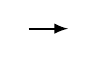
\begin{tikzpicture}[baseline = -0.5ex]
  \draw[->] (0, 0) -- (0.5, 0);
  \end{tikzpicture}  
}

% Directed dotted edge
\newcommand{\EDD}{
  \begin{tikzpicture}[baseline = -0.5ex]
  \draw[->, dotted] (0, 0) -- (0.5, 0);
  \end{tikzpicture}
}

%Análisis léxico
\newcommand{\str}[1]{\textbf{\texttt{#1}}}
\newcommand{\dash}{\text{--}}

%Recuadros
\definecolor{FondoRecuadro}{rgb}{0.90,0.90,1.0}
\makeatletter
\newenvironment{recuadro}{%
  \noindent%
  \begin{lrbox}{\@tempboxa}\begin{minipage}{\columnwidth}}{\end{minipage}\end{lrbox}%
  \colorbox{FondoRecuadro}{\usebox{\@tempboxa}}
}
\makeatother

%----Pseudocódigo---------------------------------------------------------------
\SetKwProg{Function}{función}{:}{}
\SetKwIF{If}{ElseIf}{Else}{si}{:}{en otro caso, si}{en otro caso:}{}
\SetKwFor{For}{para}{:}{}
\SetKwFor{While}{repetir mientras}{:}{}
\SetKwRepeat{Repeat}{repetir:}{hasta que}{}
\SetKwFor{ForEach}{para cada}{:}{}
\SetKw{KwFrom}{desde}
\SetKw{KwTo}{hasta}
\SetKw{Return}{devolver}
\SetKw{New}{nuevo}
\SetKw{KwAnd}{y}
\SetKw{KwAndE}{e}
\SetKw{KwOr}{o}
\SetKw{KwNot}{no}
\SetKw{Print}{imprimir}
\SetKwComment{tcp}{$\blacktriangleright$}{}
\SetKwInput{KwIn}{entrada}
\SetKwInput{KwOut}{salida}
\newcommand{\None}{\textsc{Ninguno}}
\newcommand{\False}{\textsc{Falso}}
\newcommand{\True}{\textsc{Verdadero}}

\begin{document}
\title[Clasificación Dynkin]{La clasificación Dynkin en perspectiva 
computacional}

\author[M. Abarca]{Claudia Pérez Ruisánchez\\ Mario Alberto Abarca Sotelo\\
Daniel Rivera López}

\institute[UAEM]{
Universidad Autónoma del Estado de Morelos}

\date{21 de junio de 2017}

\makebeamertitle

\pgfdeclareimage[height=0.5cm]{institution-logo}{logoUAEM}
\logo{\pgfuseimage{institution-logo}}

\AtBeginSubsection[]{%
  \frame<beamer>{ 
    \frametitle{Índice}   
    \tableofcontents[currentsection, currentsubsection] 
  }
}

%\beamerdefaultoverlayspecification{<+->}

\begin{frame}{Índice}
  \tableofcontents{}
\end{frame}

\section{La Clasificación $\DynA$-$\DynD$-$\DynE$}

\subsection{Conceptos y relaciones}
%\begin{frame}{Objetos de estudio}
%  \begin{columns}
%    \begin{column}{5cm}
%      ``\emph{Los diagramas de Dynkin-Coexeter $\DynA_k$, $\DynD_k$, 
%      $\DynE_k$ aparecen en muchos teoremas independientes de 
%      clasificación.}'' \newline
%      (Vladimir Arnold)
%    \end{column}
%    \begin{column}{5cm}
%      \includegraphics[height=1\textwidth]{Figuras/conceptos}      
%    \end{column}
%  \end{columns}
%\end{frame}

\begin{frame}{Matriz de Cartan simétrica}
  \begin{columns}
    \begin{column}{5cm}
        \begin{definition}
          \begin{itemize}
            \item<+->  Una matriz $\mat{A} \in \MatrixSet{\Zset}$ es 
            \alert{casi Cartan } si $\mat{A}$ es simétrica y $\entry{\mat{A}}{i}{i} = 2$ para toda $i = 1, \ldots, n$.
            \item<+-> Se denota por $\sqCclass$ a la clase de todas las 
            matrices 
            casi-Cartan simétricas.
          \end{itemize}      
        \end{definition}
    \end{column}
    \begin{column}{5cm}
      \begin{example}<+->
        \begin{equation*}
        \begin{pmatrix}
        2 & -2 & 1 & 0\\
        -2 & 2 & -1 & 0\\
        1 & -1 & 2 & 1\\
        0 & 0 & 1 & 2\\
        \end{pmatrix}
        \end{equation*}
      \end{example}
    \end{column}
  \end{columns}
\end{frame}

%\begin{frame}{Bigráfica}
%  \begin{columns}
%    \begin{column}{5cm}
%      \begin{definition}<+->
%        Una \alert{bigráfica} es una multigráfica $G = \Tuple{V, E}$ con 
%        bipartición en las aristas $E = E^+ \cup E^-$.
%      \end{definition}
%      \begin{itemize}
%        \item<+-> $E^+$: aristas \emph{punteadas}
%        \item<+-> $E^-$: aristas \emph{sólidas}
%      \end{itemize}
%    \end{column}
%    \begin{column}{5cm}
%      \begin{example}<+->
%        \centering
%        \begin{tikzpicture}[baseline = (v3.base), scale = 1.5]
%        \node (v1) at (-0.8604975358129109, -0.4070708333164735) {$1$};
%        \node (v2) at (-0.6144076010236877, 0.5397895385876869) {$2$};
%        \node (v3) at (0.14142321122027776, -0.13585990909663623) {$3$};
%        \node (v4) at (1.1732333853473758, -0.43758645858272716) {$4$};
%        \begin{pgfonlayer}{bg}
%        \draw[double, double distance = 0.5ex] (v1) -- (v2);
%        \draw[dotted] (v1) -- (v3);
%        \draw (v2) -- (v3);
%        \draw[dotted] (v3) -- (v4);
%        \end{pgfonlayer}
%        \end{tikzpicture}
%        \begin{align*}
%          V &= \Set{1, 2, 3, 4} \\
%          E^+ &= \Set{\Set{1, 3}, \Set{3, 4}} \\
%          E^- &= \Set{\Set{1, 2}, \Set{1, 2}, \Set{2, 3}}
%        \end{align*}
%      \end{example}
%    \end{column}
%  \end{columns}
%\end{frame}

%\begin{frame}{Forma unitaria}
%  \begin{definition}<+->
%    Una \alert{forma cuadrática unitaria} (o simplemente \emph{forma unitaria}) 
%    es un polinomio $q:\Zset^n \to \Zset$ de la forma
%    \begin{equation*}
%      q\left(x_1,\ldots,x_n\right) = \sum_{k = 1}^{n} x_k^2 + \sum_{1 \le i < j 
%      \le n} c_{i \, j} x_i x_j
%    \end{equation*}
%    con coeficientes $c_{i\,j} \in \Zset$ para toda $1 \le i < j \le n$.
%  \end{definition}
%  \begin{example}<+->
%    \begin{equation*}
%      q\left(x, y, z, w\right) = x^2 + y^2 + z^2 + w^2 - 2 x y + x z - y z + z w
%    \end{equation*}
%  \end{example}
%\end{frame}

\begin{frame}{Forma unitaria asociada a una matriz casi Cartan}
  \framesubtitle{Matriz casi-Cartan simétrica $\leftrightarrow$ Forma unitaria}
  \begin{align*}
    \Quadratic{\mat{A}}\left(\vec{x}\right) &= \frac{1}{2} 
    \transpose{\vec{x}} \mat{A} \vec{x}  %\\
    %&= \frac{1}{2} \left( \sum_{i = 1}^{n} \sum_{j = 1}^{n} 
    %   \entry{\mat{A}}{i}{j} x_i x_j \right)  \\
    %&= \frac{1}{2} \left(\sum_{i=1}^{n} \entry{\mat{A}}{i}{i} x_i^2
    %   + 2 \sum_{1 \le i < j \le n} \entry{\mat{A}}{i}{j} x_i x_j\right)  
       %\\
    %&= \sum_{i=1}^{n} x_i^2 + \sum_{1 \le i < j \le n} \entry{\mat{A}}{i}{j}    
   %    x_i x_j \text{.}
  \end{align*}
\end{frame}

\begin{frame}{Forma unitaria asociada a una matriz casi Cartan}
  \framesubtitle{Matriz casi-Cartan simétrica $\leftrightarrow$ Forma unitaria}
  \begin{align*}
    \Quadratic{\mat{A}}\left(\vec{x}\right) &= \frac{1}{2} 
    \transpose{\vec{x}} \mat{A} \vec{x}  \\
    &= \frac{1}{2} \left( \sum_{i = 1}^{n} \sum_{j = 1}^{n} 
      \entry{\mat{A}}{i}{j} x_i x_j \right)  %\\
    %&= \frac{1}{2} \left(\sum_{i=1}^{n} \entry{\mat{A}}{i}{i} x_i^2
    %   + 2 \sum_{1 \le i < j \le n} \entry{\mat{A}}{i}{j} x_i x_j\right)  
       %\\
    %&= \sum_{i=1}^{n} x_i^2 + \sum_{1 \le i < j \le n} \entry{\mat{A}}{i}{j}    
   %    x_i x_j \text{.}
  \end{align*}
\end{frame}

\begin{frame}{Forma unitaria asociada a una matriz casi Cartan}
  \framesubtitle{Matriz casi-Cartan simétrica $\leftrightarrow$ Forma unitaria}
  \begin{align*}
    \Quadratic{\mat{A}}\left(\vec{x}\right) &= \frac{1}{2} 
    \transpose{\vec{x}} \mat{A} \vec{x}  \\
    &= \frac{1}{2} \left( \sum_{i = 1}^{n} \sum_{j = 1}^{n} 
      \entry{\mat{A}}{i}{j} x_i x_j \right)  \\
    &= \frac{1}{2} \left(\sum_{i=1}^{n} \entry{\mat{A}}{i}{i} x_i^2
       + 2 \sum_{1 \le i < j \le n} \entry{\mat{A}}{i}{j} x_i x_j\right)  
       %\\
    %&= \sum_{i=1}^{n} x_i^2 + \sum_{1 \le i < j \le n} \entry{\mat{A}}{i}{j}    
   %    x_i x_j \text{.}
  \end{align*}
\end{frame}

\begin{frame}{Forma unitaria asociada a una matriz casi Cartan}
  \framesubtitle{Matriz casi-Cartan simétrica $\leftrightarrow$ Forma unitaria}
  \begin{align*}
    \Quadratic{\mat{A}}\left(\vec{x}\right) &= \frac{1}{2} 
    \transpose{\vec{x}} \mat{A} \vec{x}  \\
    &= \frac{1}{2} \left( \sum_{i = 1}^{n} \sum_{j = 1}^{n} 
      \entry{\mat{A}}{i}{j} x_i x_j \right)  \\
    &= \frac{1}{2} \left(\sum_{i=1}^{n} \entry{\mat{A}}{i}{i} x_i^2
       + 2 \sum_{1 \le i < j \le n} \entry{\mat{A}}{i}{j} x_i x_j\right)  
       \\
    &= \sum_{i=1}^{n} x_i^2 + \sum_{1 \le i < j \le n} \entry{\mat{A}}{i}{j}    
       x_i x_j \text{.}
  \end{align*}
\end{frame}

%\begin{frame}{Forma unitaria asociada a una matriz casi Cartan}
 % \framesubtitle{Matriz casi-Cartan simétrica $\leftrightarrow$ Forma unitaria}
 % \begin{align*}
 %   \Quadratic{\mat{A}}\left(\vec{x}\right) &= \frac{1}{2} 
  %  \transpose{\vec{x}} \mat{A} \vec{x}  \\
    %&= \frac{1}{2} \left( \sum_{i = 1}^{n} \sum_{j = 1}^{n} 
    %  \entry{\mat{A}}{i}{j} x_i x_j \right)  \\
    %&= \frac{1}{2} \left(\sum_{i=1}^{n} \entry{\mat{A}}{i}{i} x_i^2
     %  + 2 \sum_{1 \le i < j \le n} \entry{\mat{A}}{i}{j} x_i x_j\right)  
 %   &= \sum_{i=1}^{n} x_i^2 + \sum_{1 \le i < j \le n} \entry{\mat{A}}{i}{j}    
%       x_i x_j \text{.}
  %\end{align*}
  %\begin{definition}
  %Una matriz casi Cartan simétrica $A$ es \alert{definida positiva} si y sólo si $ \Quadratic{\mat{A}}\left(\vec{x}\right) &= \frac{1}{2} \transpose{\vec{x}} \mat{A} % \vec{x}>0$, para toda $x\in \Z$ con $x\neq \vec{0}$.
%  \end{definition}
%\end{frame}


\begin{frame}{Bigráfica asociada a una matriz casi Cartan}
  \framesubtitle{Matriz casi-Cartan simétrica $\leftrightarrow$ Bigráfica}
  \begin{theorem}
    Sea $A\in M_{n}(\mathbb{Z})$ una matriz casi Cartan simétrica y definida positiva sean  $i,j\in\{1,2...n\}$, entonces 
\begin{enumerate}
\item [$(a)$] $0\leq A_{ij}A_{ji}<4$ 
\item [$(b)$] $A_{ij}\in\{-1,0,-1\}$\end{enumerate}  \end{theorem}
La bigráfica $\Bigraph{\mat{A}}$ asociada a la matriz $A$  tiene  vértices $\left\{ 1,2,\ldots,n\right\} $, y para cada par de vértices $i$, $j$ con $i\neq j$:
	\begin{enumerate}
		\item Si $A_{ij}=-1=A_{ji}$ trazamos una arista solida entre los vértices,
		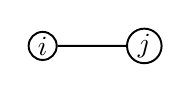
\begin{tikzpicture}[baseline = (v1.base), scale = 1.5]
      \node (v1) at (-0.8604975358129109, -0.4070708333164735) {$i$};   
      \node (v2) at (0.000, -0.4070708333164735) {$j$};
      \draw (v1)--(v2);  
       \end{tikzpicture}
		\item Si $A_{ij}=1=A_{ji}$ trazamos una arista punteada entre los vértices, 
		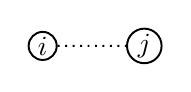
\begin{tikzpicture}[baseline = (v1.base), scale = 1.5]
      \node (v1) at (-0.8604975358129109, -0.4070708333164735) {$i$};   
      \node (v2) at (0.000, -0.4070708333164735) {$j$};
      \draw[dotted] (v1)--(v2);  
       \end{tikzpicture}
	\end{enumerate}
 \end{frame}

\begin{frame}{Equivalencia de conceptos}
  \framesubtitle{Ejemplo}
  $\mat{A} =
  \begin{pmatrix}
    2 & -2 & 1 & 0\\
    -2 & 2 & -1 & 0\\
    1 & -1 & 2 & 1\\
    0 & 0 & 1 & 2\\
  \end{pmatrix}$
  \qquad
  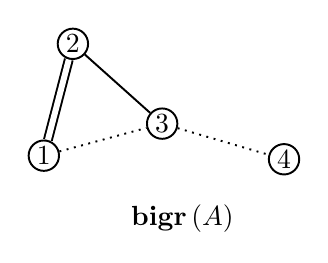
\begin{tikzpicture}[baseline = (v3.base), scale = 1.5]
    \node (v1) at (-0.8604975358129109, -0.4070708333164735) {$1$};
    \node (v2) at (-0.6144076010236877, 0.5397895385876869) {$2$};
    \node (v3) at (0.14142321122027776, -0.13585990909663623) {$3$};
    \node (v4) at (1.1732333853473758, -0.43758645858272716) {$4$};
    \begin{pgfonlayer}{bg}
    \draw[double, double distance = 0.5ex] (v1) -- (v2);
    \draw[dotted] (v1) -- (v3);
    \draw (v2) -- (v3);
    \draw[dotted] (v3) -- (v4);
    \end{pgfonlayer}
    \node[draw = none, shape = rectangle] (t) at (0.31273585,-0.937586459) 
    {$\Bigraph{\mat{A}}$};
  \end{tikzpicture}
  \begin{equation*}
    \Quadratic{\mat{A}}\left(x_1, x_2, x_3, x_4\right) = x_1^2 + x_2^2 + x_3^2 
    + x_4^2 - 2 x_1 x_2 + x_1 x_3 - x_2 x_3 + x_3 x_4
  \end{equation*}
\end{frame}

\begin{frame}{$\Zset$-equivalencia}
  \begin{definitions}
    \begin{itemize}
      \item<+-> Una matriz $\mat{M} \in \MatrixSet{\Zset}$ es 
        \alert{\Zset-invertible} si tiene inversa $\mat{M}^{-1} \in 
        \MatrixSet{\Zset}$.
      \item<+-> $\mat{A}, \mat{A^{\prime}} \in \sqCclass$ son 
      \alert{\Zset-equivalentes} si existe una matriz $\Zset$-invertible 
      $\mat{M}$ tal que $\mat{A}^\prime = \transpose{\mat{M}} \mat{A} \mat{M}$.
    \end{itemize}
  \end{definitions}
\end{frame}

\begin{frame}{Diagramas de Dynkin}
  \begin{itemize}
    \item Todas las bigráficas conexas, definidas positivas, de aristas sólidas:
  \end{itemize}
  \pause
  \begin{tabular}{ll}
    Familia & Gráfica\\
    $\DynA_{n}$, $n\ge1$ &
    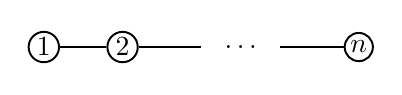
\begin{tikzpicture}
    [baseline=(v1.base)]
    \node (v1) at (0, 0) {$1$};
    \node (v2) at (1, 0) {$2$};
    \node (v3) at (4, 0) {$n$};
    \node[draw = none] (v5) at (2.5, 0) {$\ldots$};
    \draw (v1) -- (v2) -- (2, 0);
    \draw (3, 0) -- (v3);
    \end{tikzpicture} \pause \\
    $\DynD_{n}$, $n\ge4$ &
    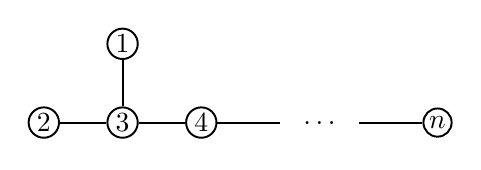
\begin{tikzpicture}
    [baseline=(v1.base)]
    \node (v1) at (0, 0) {$2$};
    \node (v2) at (1, 0) {$3$};
    \node (v3) at (2, 0) {$4$};
    \node (v4) at (5, 0) {$n$};
    \node (v5) at (1, 1) {$1$};
    \node[draw = none] (dots) at (3.5, 0) {$\ldots$};
    \draw (v1) -- (v2) -- (v3) -- (3, 0); \draw (v5)
    -- (v2); \draw (4, 0) -- (v4);
    \end{tikzpicture}\pause \\
    $\DynE_{n}$, $6\le n\le8$ &
    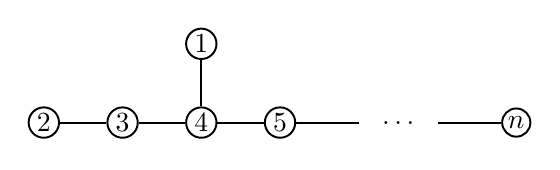
\begin{tikzpicture} [baseline=(v1.base)]
    \node (v1) at (0, 0) {$2$};
    \node (v2) at (1, 0) {$3$};
    \node (v3) at (2, 0) {$4$};
    \node (v4) at (3, 0) {$5$};
    \node (v5) at (6, 0) {$n$};
    \node (v6) at (2, 1) {$1$};
    \node[draw = none] (dots) at (4.5, 0) {$\ldots$};
    \draw (v1) -- (v2) -- (v3) -- (v4) -- (4, 0);
    \draw (v6) -- (v3);
    \draw (5, 0) -- (v5);
    \end{tikzpicture}\\
  \end{tabular}
\end{frame}

\begin{frame}{La clasificación \DynA-\DynD-\DynE}
  \begin{theorem}<+->[S. Ovsienko -- 1978]
    Toda bigráfica $G$ definida positiva es \Zset-equivalente a una bigráfica 
    sin aristas punteadas, que está determinada de forma única hasta 
    isomorfismo de gráficas, y es la unión disjunta de diagramas de Dynkin.
  \end{theorem}
  \begin{itemize}
    \item<+-> Demostración constructiva llamada \alert{algoritmo de las 
    inflaciones}.
  \end{itemize}
\end{frame}

\subsection{Algoritmo de las inflaciones}
\begin{frame}{Inflaciones}
  \begin{definitions}
    \begin{itemize}[<+->]
      \item $\mat{I}$ denota la matriz identidad con vectores columna 
      $\vec{e}_j$.
      \item $\Elementary{s}{r}{\sigma} \defeq \mat{I} + \sigma \, \vec{e}_s \, 
      \transpose{\vec{e}_r}$ ($s, r \in \Set{1, \ldots, n}$, $\sigma \in 
      \Rset$) denota una \alert{matriz elemental} de suma de renglones/columnas.
      \item Si $\mat{A} \in \sqCclass$ y $\entry{\mat{A}}{s}{r} = 1$ entonces 
      $\transpose{\left(\Elementary{s}{r}{-1}\right)} \mat{A} 
      \left(\Elementary{s}{r}{-1}\right)$ es una \alert{inflación} de $\mat{A}$.
    \end{itemize}
  \end{definitions}
\end{frame}

\begin{frame}{Algoritmo de las inflaciones}
  \begin{block}{Algoritmo de las inflaciones}<+->
  \SetKwFunction{Inflaciones}{inflaciones}
    \begin{algorithm}[H]
      \Function{\Inflaciones{$\mat{A}$}}{
        \While{exista una entrada no diagonal $\entry{\mat{A}}{s}{r} = 1$}{
          $\mat{A} \gets \transpose{\left(\Elementary{s}{r}{-1}\right)} \, 
          \mat{A} 
          \, \left(\Elementary{s}{r}{-1}\right)$
        }
      }
    \end{algorithm}
  \end{block}
  \begin{itemize}[<+->]
    \item Se justifica en que $\abs{\Quadratic{\mat{A}}^{-1}\left(1\right)} < 
    \infty$ permanece constante en cada iteración mientras que 
    $\abs{\Quadratic{\mat{A}}^{-1}\left(1\right)\cap\Nset^n}$ crece.
    \item Cota superior del número de raíces positivas $\bigOh{n \cdot 6^{n}}$ (Kosakowska -- 2012).
  \end{itemize}
\end{frame}

\subsection{Las construcciones de Barot}

\begin{frame}{El caso $\mathbb{A}_n$}
  \begin{columns}
    \begin{column}{5cm}
      \emph{Los $\mathbb{A}$-bloques.}
    \end{column}
    \begin{column}{5cm}
      \includegraphics[height=1\textwidth]{Figuras/A-bloque1}      
    \end{column}
  \end{columns}
\end{frame}

\begin{frame}{El caso $\mathbb{A}_n$}
  \begin{columns}
    \begin{column}{5cm}
      \includegraphics[height=1\textwidth]{Figuras/A-bloque1} 
    \end{column}
    \begin{column}{5cm}
      \includegraphics[height=1\textwidth]{Figuras/A-bloque2}      
    \end{column}
  \end{columns}
\end{frame}

\begin{frame}{El caso $\mathbb{A}_n$}
  \begin{columns}
    \begin{column}{5cm}
      \includegraphics[height=1\textwidth]{Figuras/A-bloque2} 
    \end{column}
    \begin{column}{5cm}
      \includegraphics[height=1\textwidth]{Figuras/A-bloque3}      
    \end{column}
  \end{columns}
\end{frame}


\begin{frame}{La condición de ciclo}
  \begin{columns}
    \begin{column}{0.5\textwidth}
      \begin{itemize}[<+->]
        \item Convención: Una pareja de aristas paralelas se considera un ciclo 
        de longitud 2.
      \end{itemize}
      \begin{definition}<+->
        Una bigráfica cumple la \alert{condición de ciclo} si todo ciclo sin 
        cuerdas tiene un número impar de aristas punteadas.
      \end{definition}
    \end{column}
    \begin{column}{0.5\textwidth}
      \begin{example}<+->
        \centering
        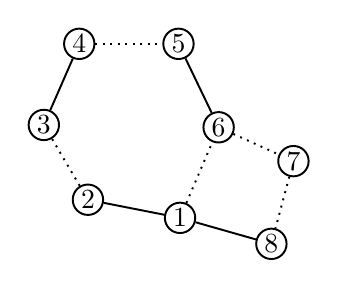
\begin{tikzpicture}
        \node (v0) at (0.07, -1.09) {1};
        \node (v1) at (-1.1, -0.86) {2};
        \node (v2) at (-1.66, 0.09) {3};
        \node (v3) at (-1.21, 1.12) {4};
        \node (v4) at (0.05, 1.12) {5};
        \node (v5) at (0.56, 0.06) {6};
        \node (v6) at (1.51, -0.37) {7};
        \node (v7) at (1.23, -1.42) {8};
        \draw[dotted] (v0) -- (v5);
        \draw (v0) -- (v1);
        \draw (v0) -- (v7);
        \draw[dotted] (v1) -- (v2);
        \draw (v2) -- (v3);
        \draw[dotted] (v3) -- (v4);
        \draw (v4) -- (v5);
        \draw[dotted] (v5) -- (v6);
        \draw[dotted] (v6) -- (v7);
        \end{tikzpicture}
      \end{example}
    \end{column}
  \end{columns}
\end{frame}

\begin{frame}{El marco de una bigráfica}
  \begin{columns}
    \begin{column}{0.5\textwidth}
      \begin{definition}<+->
        El \alert{marco} $\Marco{G}$ de una bigráfica $G$ es su gráfica 
        subyacente.
      \end{definition}
      \begin{itemize}[<+->]
        \item Su diagrama se obtiene reemplazando aristas punteadas por sólidas.
      \end{itemize}
    \end{column}
    \begin{column}{0.5\textwidth}
      \begin{example}<+->
        \centering
        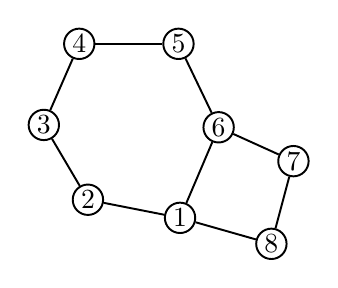
\begin{tikzpicture}
        \node (v0) at (0.07, -1.09) {1};
        \node (v1) at (-1.1, -0.86) {2};
        \node (v2) at (-1.66, 0.09) {3};
        \node (v3) at (-1.21, 1.12) {4};
        \node (v4) at (0.05, 1.12) {5};
        \node (v5) at (0.56, 0.06) {6};
        \node (v6) at (1.51, -0.37) {7};
        \node (v7) at (1.23, -1.42) {8};
        \draw (v0) -- (v5);
        \draw (v0) -- (v1);
        \draw (v0) -- (v7);
        \draw (v1) -- (v2);
        \draw (v2) -- (v3);
        \draw (v3) -- (v4);
        \draw (v4) -- (v5);
        \draw (v5) -- (v6);
        \draw (v6) -- (v7);
        \end{tikzpicture}
      \end{example}
    \end{column}
  \end{columns}
\end{frame}

\begin{frame}{Ensamblaje de árbol}
  \begin{block}{Construcción (ensamblaje de árbol)}
    \textbf{Datos:}
    \begin{itemize}[<+->]
      \item un árbol $T$ con $\VertexSet{T} = \Set{1, 2, \ldots, t}$;
      \item $t$ bigráficas $B_1, B_2, \ldots, B_t$;
      \item para cada $i \in \VertexSet{G}$ una función inyectiva $\sigma_i : 
      \frontier[T]{i} \to \VertexSet{B_i}$.
    \end{itemize}
    \textbf{Procedimiento:}
    \begin{enumerate}[<+->]
      \item calcular la unión disjunta  $H = B_1 \sqcup B_2 \sqcup \cdots 
      \sqcup B_t$;
      \item para cada $e = \Set{i, j} \in \EdgeSet{T}$ identificar 
      $\sigma_i\left(e\right) = \sigma_j\left(e\right)$ en $H$.
    \end{enumerate}
  \end{block}
\end{frame}

\begin{frame}{Construcción de $\DynA_n$}
  \begin{theorem}[M. Barot -- 1999]
    Una bigráfica $G$ es de tipo Dynkin $\DynA$ si y sólo si satisface la 
    condición de ciclo y $\Marco{G}$ es un ensamblaje de árbol de gráficas 
    completas.
  \end{theorem}
\end{frame}

\begin{frame}{Construcción de $\DynA_n$}
  \framesubtitle{Ejemplo}
  \begin{columns}
    \begin{column}{0.5\textwidth}
      \begin{equation*}
        T =
        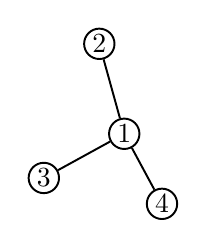
\begin{tikzpicture}[scale = 0.8, baseline = (B2.base)]
          \node (B1) at (0.9882314470711424, 0.022706017651931643) {$1$};
          \node (B2) at (0.5923935348744648, 1.4508406462539858) {$2$};
          \node (B3) at (-0.2884249194391753, -0.6784940273952205) {$3$};
          \node (B4) at (1.5875974862305025, -1.0893921745565085) {$4$};
          \draw (B2) -- (B1) -- (B3);
          \draw (B1) -- (B4);
        \end{tikzpicture}
      \end{equation*}
      \begin{align*}
        B_1 &= K_4\\
        B_2 &= K_3\\
        B_3 &= K_3\\
        B_4 &= K_2\\
      \end{align*}
    \end{column}
    \begin{column}{0.5\textwidth}
      \begin{align*}
        \sigma_1 &= \begin{pmatrix}
          \Set{1, 2} & \Set{1, 3} & \Set{1, 4}\\
          1          & 3          & 2\\
        \end{pmatrix}\\
        \sigma_2 &= \begin{pmatrix}
          \Set{1, 2}\\
          3
        \end{pmatrix}\\
        \sigma_3 &= \begin{pmatrix}
          \Set{1, 3}\\
          1
        \end{pmatrix}\\
        \sigma_4 &= \begin{pmatrix}
          \Set{1, 4}\\
          1
        \end{pmatrix}
      \end{align*}
    \end{column}
  \end{columns}
\end{frame}

\begin{frame}{Construcción de $\DynA_n$}
  \framesubtitle{Ejemplo (continuado)}
  \begin{columns}
    \begin{column}{0.5\textwidth}
      \begin{equation*}
      H = 
      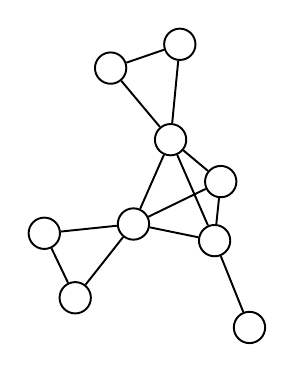
\begin{tikzpicture}[baseline = (v1.base), every node/.style={inner 
        sep=4pt, circle, draw}]
      \node (v1) at (0.045723322887135334, 1.6531597581429232) {};
      \node (v2) at (0.924316069611771, 1.9552990371412833) {};
      \node (v3) at (0.807141212124488, 0.7440631434777515) {};
      \node (v4) at (1.366122335327793, -0.5380224344255913) {};
      \node (v5) at (0.335701115736255, -0.32692551580387064) {};
      \node (v6) at (-0.7967889893835305, -0.4447190885953058) {};
      \node (v7) at (1.809072637133212, -1.6407619146874255) {};
      \node (v8) at (-0.4041868846702505, -1.263837477786485) {};
      \node (v9) at (1.4439611250960338, 0.21170887735943703) {};
      \draw (v1) -- (v2);
      \draw (v1) -- (v3);
      \draw (v2) -- (v3);
      \draw (v3) -- (v4);
      \draw (v3) -- (v5);
      \draw (v3) -- (v9);
      \draw (v4) -- (v5);
      \draw (v4) -- (v7);
      \draw (v4) -- (v9);
      \draw (v5) -- (v6);
      \draw (v5) -- (v8);
      \draw (v5) -- (v9);
      \draw (v6) -- (v8);
      \end{tikzpicture}
      \end{equation*}
    \end{column}
    \begin{column}{0.5\textwidth}
      \begin{equation*}
      G = 
      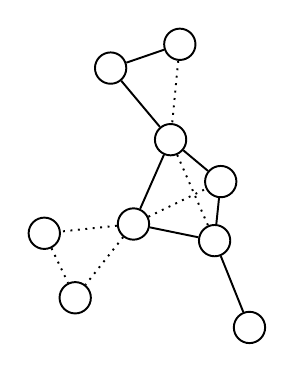
\begin{tikzpicture}[baseline = (v1.base), every node/.style={inner 
        sep=4pt, circle, draw}]
      \node (v1) at (0.045723322887135334, 1.6531597581429232) {};
      \node (v2) at (0.924316069611771, 1.9552990371412833) {};
      \node (v3) at (0.807141212124488, 0.7440631434777515) {};
      \node (v4) at (1.366122335327793, -0.5380224344255913) {};
      \node (v5) at (0.335701115736255, -0.32692551580387064) {};
      \node (v6) at (-0.7967889893835305, -0.4447190885953058) {};
      \node (v7) at (1.809072637133212, -1.6407619146874255) {};
      \node (v8) at (-0.4041868846702505, -1.263837477786485) {};
      \node (v9) at (1.4439611250960338, 0.21170887735943703) {};
      \draw (v1) -- (v2);
      \draw (v1) -- (v3);
      \draw[dotted] (v2) -- (v3);
      \draw[dotted] (v3) -- (v4);
      \draw (v3) -- (v5);
      \draw (v3) -- (v9);
      \draw (v4) -- (v5);
      \draw (v4) -- (v7);
      \draw (v4) -- (v9);
      \draw[dotted] (v5) -- (v6);
      \draw[dotted] (v5) -- (v8);
      \draw[dotted] (v5) -- (v9);
      \draw[dotted] (v6) -- (v8);
      \end{tikzpicture}
      \end{equation*}
    \end{column}
  \end{columns}
\end{frame}

\begin{frame}{Construcciones para $\DynD_n$}
  \begin{block}{Construcción (extensión de $\DynA$-espejo)}
    \textbf{Datos:}
    \begin{itemize}[<+->]
      \item una gráfica $G$ que haya sido obtenida mediante un ensamblaje de 
      árbol de gráficas completas;
      \item un vértice $x\in V\left(G\right)$.
    \end{itemize}
    \textbf{Instrucciones:}
    \begin{enumerate}[<+->]
      \item agregar un nuevo vértice $x^\prime$ a $G$;
      \item para cada $y$ vecino de $x$ agregar una arista $\Set{x^\prime, y}$ 
      a $G$.
    \end{enumerate}
  \end{block}
\end{frame}

\begin{frame}{Construcciones para $\DynD_n$}
  \begin{block}{Construcción ($\DynA$-ciclado)}
    \textbf{Datos:}
    \begin{itemize}[<+->]
      \item una gráfica $G$ que haya sido obtenido mediante un ensamblaje de 
      árbol de gráficas completas;
      \item dos vértices $x, y \in \VertexSet{G}$ a distancia $d_{G}\left(x, 
      y\right) \ge 3$.
    \end{itemize}
    \textbf{Instrucciones:}
    \begin{enumerate}[<+->]
      \item identificar $x = y$ en $G$.
    \end{enumerate}
  \end{block}
\end{frame}

\begin{frame}{Ejemplos}
  \begin{equation*}
  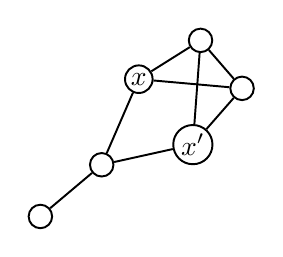
\begin{tikzpicture}[baseline = (current bounding box.center), every 
  node/.style={inner sep=3pt, draw, circle}]
  \node[inner sep=1pt] (v1) at (-0.17702807361217932, 
  0.2169077993202585) {$x$};
  \node[inner sep=1pt] (v2) at (0.5094847697505441, 
  -0.6140803384090112) {$x^\prime$};
  \node (v3) at (0.6069997477997765, 0.7096309089544152) {};
  \node (v4) at (1.1343769499172704, 0.10036276119312261) {};
  \node (v5) at (-0.648145832261598, -0.8701436995030774) {};
  \node (v6) at (-1.4270078527724706, -1.5265337186469214) {};
  \draw (v1) -- (v3);
  \draw (v1) -- (v4);
  \draw (v1) -- (v5);
  \draw (v2) -- (v3);
  \draw (v2) -- (v4);
  \draw (v2) -- (v5);
  \draw (v3) -- (v4);
  \draw (v5) -- (v6);
  \end{tikzpicture}
  \qquad
  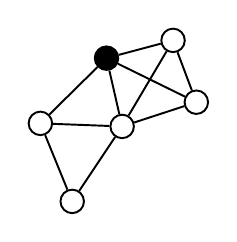
\begin{tikzpicture}[baseline = (current bounding box.center), every 
  node/.style={inner sep=3pt, draw, circle}]
  \node (v1) at (-0.2814306111671281, 0.8990219271931051) {};
  \node (v2) at (0.75691323601581, 0.8600382799848384) {};
  \node[fill = black, text = white] (v3) at (0.5586925858271716, 
  1.7274992556341786) {};
  \node (v4) at (1.6988576401743483, 1.1678621669884481) {};
  \node (v5) at (1.4035768281579486, 1.9530041708564487) {};
  \node (v6) at (0.12280539183944258, -0.09186288489949457) {};
  \draw (v1) -- (v2);
  \draw (v1) -- (v3);
  \draw (v1) -- (v6);
  \draw (v2) -- (v3);
  \draw (v2) -- (v4);
  \draw (v2) -- (v5);
  \draw (v2) -- (v6);
  \draw (v3) -- (v4);
  \draw (v3) -- (v5);
  \draw (v4) -- (v5);
  \end{tikzpicture}
  \end{equation*}
\end{frame}

\begin{frame}{Construcción de $\DynD_n$}
  \begin{theorem}[M. Barot - 2001]
    Una bigráfica $G$ es de tipo $\DynD$ si y sólo si las siguientes tres 
    condiciones se satisfacen:
    \begin{enumerate}[<+->]
      \item $G$ tiene cuatro o más vértices
      \item $G$ cumple la condición de ciclo
      \item $\Marco{G}$ se obtiene mediante una extensión de 
      $\DynA$-espejo o un $\DynA$-ciclado.
    \end{enumerate}
  \end{theorem}
\end{frame}

\subsection{Planteamiento}
\begin{frame}{Planteamiento}
  \begin{itemize}[<+->]
    \item ¿Qué \alert{técnicas computacionales} se pueden aplicar para el 
    estudio de la clasificación \DynA-\DynD-\DynE?
    \item ¿Qué \alert{criterios eficientes} se pueden aplicar para clasificar 
    una bigráfica?
    \item ¿Qué \alert{complejidad computacional} tiene el problema de 
    clasificar una bigráfica?
  \end{itemize}
\end{frame}

\section{Aportaciones en perspectiva computacional}

\subsection{El morfismo de flación y sus invariantes}
\begin{frame}{Motivación}
    Para estudiar un algoritmo se suele identificar qué atributos cambian o 
    permanecen invariantes a lo largo de la ejecución.
\end{frame}

\begin{frame}{La flación}
  \begin{itemize}[<+->]
    \item $\mat{A}^\prime \defeq 
    \transpose{\left(\Elementary{s}{r}{\sigma}\right)} \mat{A} 
    \left(\Elementary{s}{r}{\sigma}\right)$, $\sigma \in \Rset$;
    \item $\entry{\mat{A}^\prime}{r}{r} = \entry{\mat{A}}{r}{r} + \sigma 
    \left(\entry{\mat{A}}{s}{r} + \entry{\mat{A}}{r}{s}\right) + 
    \sigma^2\entry{\mat{A}}{s}{s}$;
    \item si $\mat{A}, \mat{A}^\prime \in \sqCclass$ entonces 
    $\entry{\mat{A}^\prime}{r}{r} = 2$;
    \item entonces $\sigma \in \Set{0, -\entry{\mat{A}}{s}{r}}$.
  \end{itemize}
  \begin{definition}<+->
    Llamamos \alert{flación} al siguiente morfismo:
    \begin{equation*}
      \Flation{s}{r}{\mat{A}} \defeq 
      \transpose{\left(\Elementary{s}{r}{-\entry{\mat{A}}{s}{r}}\right)} 
      \mat{A} \left(\Elementary{s}{r}{-\entry{\mat{A}}{s}{r}}\right)\text{.}
    \end{equation*}
  \end{definition}
\end{frame}

\begin{frame}{Cómputo de una flación}
  \begin{itemize}[<+->]
    \item La flación se puede implementar en $\bigOh{n}$ operaciones.
  \end{itemize}
  \begin{block}<+->{Algoritmo}
    \SetKwFunction{Flacion}{flación}
    \begin{algorithm}[H]
      \Function{\Flacion{$\mat{A}, s, r$}}{
        $\sigma \gets -\entry{\mat{A}}{s}{r}$\;
        \For{$j = 1$ \KwTo $n$}{
          $\entry{\mat{A}}{r}{j} \gets \entry{\mat{A}}{r}{j} + \sigma 
          \entry{\mat{A}}{s}{j}$\;
        }
        \For{$i = 1$ \KwTo $n$}{
          $\entry{\mat{A}}{i}{r} \gets \entry{\mat{A}}{i}{r} + \sigma 
          \entry{\mat{A}}{i}{s}$\;%\label{li:reasignacion_rr}\;
        }
      }
    \end{algorithm}
  \end{block}
\end{frame}

\begin{frame}[label=ejemploFlacion]{Interpretación gráfica}
  \begin{example}<1->[$\Flation{1}{5}{G}$]
    \centering
    \only{
      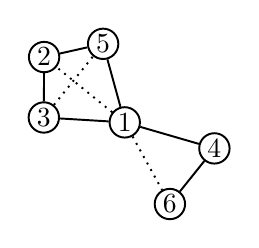
\begin{tikzpicture}
      \node (v1) at (0.5783140174240109, -0.3166613786083942) {$1$};
      \node (v2) at (-0.44575835363976835, 0.5128328399021246) {$2$};
      \node (v3) at (-0.44938111110291284, -0.2545625932461614) {$3$};
      \node (v4) at (1.7169249235942454, -0.6471916538729541) {$4$};
      \node (v5) at (0.3039359827412884, 0.6808427684519154) {$5$};
      \node (v6) at (1.1515342924415832, -1.353600447175456) {$6$};
      \draw[dotted] (v1) -- (v2);
      \draw (v1) -- (v3);
      \draw (v1) -- (v4);
      \draw (v1) -- (v5);
      \draw[dotted] (v1) -- (v6);
      \draw (v2) -- (v3);
      \draw (v2) -- (v5);
      \draw[dotted] (v3) -- (v5);
      \draw (v4) -- (v6);
      \end{tikzpicture}
    }<1>
    \only{
      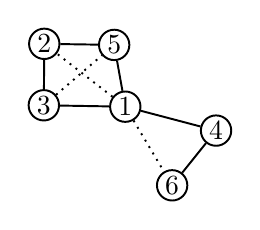
\begin{tikzpicture}
      \node (v1) at (0.5412198978114261, -0.30837975982599586) {$1$};
      \node (v2) at (-0.48785274767316644, 0.489844710272699) {$2$};
      \node (v3) at (-0.4933754862393873, -0.2907417156736922) {$3$};
      \node (v4) at (1.6939482240034156, -0.6120585870010133) {$4$};
      \node (v5) at (0.40000368649860146, 0.4762208321087451) {$5$};
      \node (v6) at (1.1362237482385447, -1.307276832397221) {$6$};
      \draw[dotted] (v1) -- (v2);
      \draw (v1) -- (v3);
      \draw (v1) -- (v4);
      \draw (v1) -- (v5);
      \draw[dotted] (v1) -- (v6);
      \draw (v2) -- (v3);
      \draw (v2) -- (v5);
      \draw[dotted] (v3) -- (v5);
      \draw (v4) -- (v6);
      \end{tikzpicture}
    }<2>
    \only{
      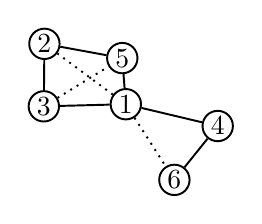
\begin{tikzpicture}
      \node (v1) at (0.5041257781988414, -0.30009814104359744) {$1$};
      \node (v2) at (-0.5299471417065647, 0.4668565806432734) {$2$};
      \node (v3) at (-0.5373698613758617, -0.3269208381012231) {$3$};
      \node (v4) at (1.670971524412586, -0.5769255201290725) {$4$};
      \node (v5) at (0.45906032004567493, 0.28561630232156) {$5$};
      \node (v6) at (1.120913204035506, -1.2609532176189864) {$6$};
      \draw[dotted] (v1) -- (v2);
      \draw (v1) -- (v3);
      \draw (v1) -- (v4);
      \draw (v1) -- (v5);
      \draw[dotted] (v1) -- (v6);
      \draw (v2) -- (v3);
      \draw (v2) -- (v5);
      \draw[dotted] (v3) -- (v5);
      \draw (v4) -- (v6);
      \end{tikzpicture}
    }<3>
    \only{
      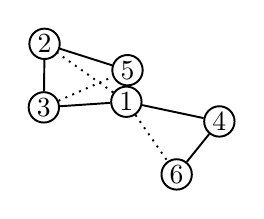
\begin{tikzpicture}
      \node (v1) at (0.4670316585862566, -0.2918165222611991) {$1$};
      \node (v2) at (-0.5720415357399629, 0.4438684510138479) {$2$};
      \node (v3) at (-0.5813642365123363, -0.36309996052875393) {$3$};
      \node (v4) at (1.647994824821756, -0.5417924532571318) {$4$};
      \node (v5) at (0.4811058833825087, 0.10902917909036036) {$5$};
      \node (v6) at (1.1056026598324675, -1.2146296028407517) {$6$};
      \draw[dotted] (v1) -- (v2);
      \draw (v1) -- (v3);
      \draw (v1) -- (v4);
      \draw (v1) -- (v5);
      \draw[dotted] (v1) -- (v6);
      \draw (v2) -- (v3);
      \draw (v2) -- (v5);
      \draw[dotted] (v3) -- (v5);
      \draw (v4) -- (v6);
      \end{tikzpicture}
    }<4>
    \only{
      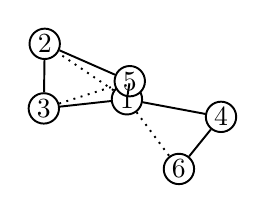
\begin{tikzpicture}
      \node (v1) at (0.4299375389736718, -0.2835349034788007) {$1$};
      \node (v2) at (-0.6141359297733611, 0.42088032138442233) {$2$};
      \node (v3) at (-0.6253586116488108, -0.39927908295628484) {$3$};
      \node (v4) at (1.6250181252309264, -0.5066593863851909) {$4$};
      \node (v5) at (0.4661403765091028, -0.05354053758485405) {$5$};
      \node (v6) at (1.090292115629429, -1.168305988062517) {$6$};
      \draw[dotted] (v1) -- (v2);
      \draw (v1) -- (v3);
      \draw (v1) -- (v4);
      \draw (v1) -- (v5);
      \draw[dotted] (v1) -- (v6);
      \draw (v2) -- (v3);
      \draw (v2) -- (v5);
      \draw[dotted] (v3) -- (v5);
      \draw (v4) -- (v6);
      \end{tikzpicture}
    }<5>
    \only{
      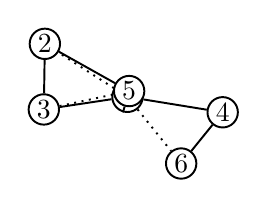
\begin{tikzpicture}
      \node (v1) at (0.3928434193610871, -0.27525328469640237) {$1$};
      \node (v2) at (-0.6562303238067592, 0.3978921917549967) {$2$};
      \node (v3) at (-0.6693529867852852, -0.43545820538381563) {$3$};
      \node (v4) at (1.6020414256400966, -0.4715263195132502) {$4$};
      \node (v5) at (0.41416379942545734, -0.20209284770408312) {$5$};
      \node (v6) at (1.0749815714263902, -1.1219823732842822) {$6$};
      \draw[dotted] (v1) -- (v2);
      \draw (v1) -- (v3);
      \draw (v1) -- (v4);
      \draw (v1) -- (v5);
      \draw[dotted] (v1) -- (v6);
      \draw (v2) -- (v3);
      \draw (v2) -- (v5);
      \draw[dotted] (v3) -- (v5);
      \draw (v4) -- (v6);
      \end{tikzpicture}
    }<6>
    \only{
      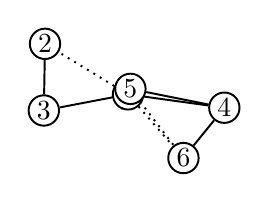
\begin{tikzpicture}
      \node (v1) at (0.35574929974850233, -0.266971665914004) {$1$};
      \node (v2) at (-0.6983247178401573, 0.37490406212557115) {$2$};
      \node (v3) at (-0.7133473619217596, -0.47163732781134654) {$3$};
      \node (v4) at (1.579064726049267, -0.4363932526413094) {$4$};
      \node (v5) at (0.3863224473654325, -0.19731558056068116) {$5$};
      \node (v6) at (1.0596710272233518, -1.0756587585060475) {$6$};
      \draw[dotted] (v1) -- (v2);
      \draw (v1) -- (v3);
      \draw (v1) -- (v4);
      \draw[dotted] (v1) -- (v5);
      \draw[dotted] (v1) -- (v6);
      \draw (v2) -- (v3);
      \draw (v4) -- (v5);
      \draw (v4) -- (v6);
      \draw[dotted] (v5) -- (v6);
      \end{tikzpicture}
    }<7>
    \only{
      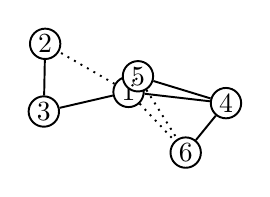
\begin{tikzpicture}
      \node (v1) at (0.31865518013591754, -0.2586900471316056) {$1$};
      \node (v2) at (-0.7404191118735555, 0.3519159324961456) {$2$};
      \node (v3) at (-0.7573417370582343, -0.5078164502388773) {$3$};
      \node (v4) at (1.5560880264584371, -0.4012601857693686) {$4$};
      \node (v5) at (0.4381329256443877, -0.060234845988625885) {$5$};
      \node (v6) at (1.044360483020313, -1.0293351437278129) {$6$};
      \draw[dotted] (v1) -- (v2);
      \draw (v1) -- (v3);
      \draw (v1) -- (v4);
      \draw[dotted] (v1) -- (v5);
      \draw[dotted] (v1) -- (v6);
      \draw (v2) -- (v3);
      \draw (v4) -- (v5);
      \draw (v4) -- (v6);
      \draw[dotted] (v5) -- (v6);
      \end{tikzpicture}
    }<8>
    \only{
      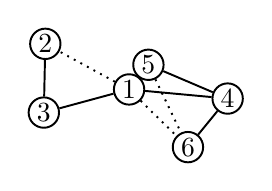
\begin{tikzpicture}
      \node (v1) at (0.2815610605233328, -0.25040842834920723) {$1$};
      \node (v2) at (-0.7825135059069537, 0.32892780286672) {$2$};
      \node (v3) at (-0.8013361121947087, -0.5439955726664083) {$3$};
      \node (v4) at (1.5331113268676075, -0.3661271188974279) {$4$};
      \node (v5) at (0.5269544741335828, 0.06282848202744401) {$5$};
      \node (v6) at (1.0290499388172745, -0.983011528949578) {$6$};
      \draw[dotted] (v1) -- (v2);
      \draw (v1) -- (v3);
      \draw (v1) -- (v4);
      \draw[dotted] (v1) -- (v5);
      \draw[dotted] (v1) -- (v6);
      \draw (v2) -- (v3);
      \draw (v4) -- (v5);
      \draw (v4) -- (v6);
      \draw[dotted] (v5) -- (v6);
      \end{tikzpicture}
    }<9>
    \only{
      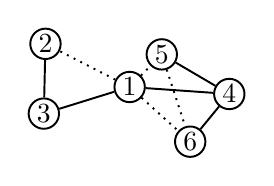
\begin{tikzpicture}
      \node (v1) at (0.24446694091074805, -0.24212680956680888) {$1$};
      \node (v2) at (-0.8246078999403518, 0.30593967323729443) {$2$};
      \node (v3) at (-0.8453304873311831, -0.5801746950939392) {$3$};
      \node (v4) at (1.5101346272767775, -0.33099405202548704) {$4$};
      \node (v5) at (0.6527870928330174, 0.17187440348752864) {$5$};
      \node (v6) at (1.013739394614236, -0.9366879141713432) {$6$};
      \draw[dotted] (v1) -- (v2);
      \draw (v1) -- (v3);
      \draw (v1) -- (v4);
      \draw[dotted] (v1) -- (v5);
      \draw[dotted] (v1) -- (v6);
      \draw (v2) -- (v3);
      \draw (v4) -- (v5);
      \draw (v4) -- (v6);
      \draw[dotted] (v5) -- (v6);
      \end{tikzpicture}
    }<10>
    \only{
      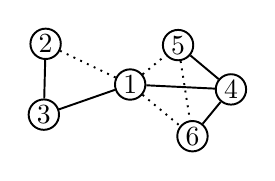
\begin{tikzpicture}
      \node (v1) at (0.2073728212981633, -0.23384519078441052) {$1$};
      \node (v2) at (-0.86670229397375, 0.2829515436078689) {$2$};
      \node (v3) at (-0.8893248624676576, -0.6163538175214699) {$3$};
      \node (v4) at (1.487157927685948, -0.2958609851535463) {$4$};
      \node (v5) at (0.8156307817426915, 0.2669029183916278) {$5$};
      \node (v6) at (0.9984288504111973, -0.8903642993931086) {$6$};
      \draw[dotted] (v1) -- (v2);
      \draw (v1) -- (v3);
      \draw (v1) -- (v4);
      \draw[dotted] (v1) -- (v5);
      \draw[dotted] (v1) -- (v6);
      \draw (v2) -- (v3);
      \draw (v4) -- (v5);
      \draw (v4) -- (v6);
      \draw[dotted] (v5) -- (v6);
      \end{tikzpicture}
    }<11>
    \only{
      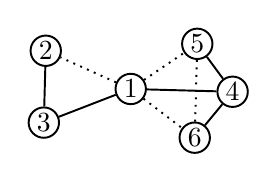
\begin{tikzpicture}
      \node (v1) at (0.17027870168557854, -0.22556357200201213) {$1$};
      \node (v2) at (-0.9087966880071481, 0.2599634139784433) {$2$};
      \node (v3) at (-0.933319237604132, -0.6525329399490009) {$3$};
      \node (v4) at (1.464181228095118, -0.2607279182816055) {$4$};
      \node (v5) at (1.0154855408626053, 0.3479140267397417) {$5$};
      \node (v6) at (0.9831183062081588, -0.8440406846148738) {$6$};
      \draw[dotted] (v1) -- (v2);
      \draw (v1) -- (v3);
      \draw (v1) -- (v4);
      \draw[dotted] (v1) -- (v5);
      \draw[dotted] (v1) -- (v6);
      \draw (v2) -- (v3);
      \draw (v4) -- (v5);
      \draw (v4) -- (v6);
      \draw[dotted] (v5) -- (v6);
      \end{tikzpicture}
    }<12>
  \end{example}
\end{frame}

\begin{frame}{Propiedades de la flación}
  \begin{lemma}<+-> Sea $G$ una bigráfica y $s, r \in \VertexSet{G}$; entonces
    \begin{enumerate}[<+->]
      \item $T_{s\,r}\left(G\right) - r = G - r$.
      \item $T_{s\,r}\left(T_{s\,r}\left(G\right)\right) = G$.
      \item Si $s \ne r$ y $\Set{s, r} \notin \EdgeSet{G}$, entonces 
      $T_{s \, r}\left( G \right) = G$.
    \end{enumerate}
  \end{lemma}
  \begin{lemma}<+->
    Sea $G$ una bigráfica con $s \in \VertexSet{G}$, y sean $r_1, r_2, \ldots, 
    r_k$ los vecinos de $s$; entonces $\Flation{s}{s}{G} = \FlationOp{s}{r_k} 
    \circ \cdots \circ \FlationOp{s}{r_2}\circ \Flation{s}{r_1}{G}$.
  \end{lemma}
\end{frame}

\begin{frame}{Invariantes de flación}
  \begin{definition}<+->
    Una propiedad de bigráficas $P$ es \alert{invariante de flación} si para 
    toda pareja $s, r \in \VertexSet{G}$ se tiene que
    \begin{equation*}
      P\left(G\right) \Rightarrow P\left(\Flation{s}{r}{G}\right)
    \end{equation*}
  \end{definition}  
  \begin{itemize}[<+->]
    \item La conexidad de una bigráfica es invariante de flación
    \item La condición de ciclo no lo es
  \end{itemize}
  \only{\phantom{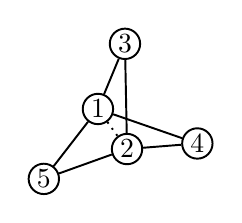
\begin{tikzpicture}
      \node (v1) at (-0.21903373405320625, 0.22955784831048787) {$1$};
      \node (v2) at (0.15063734133854118, -0.27925073637984904) {$2$};
      \node (v3) at (0.12422593618363328, 1.0570054168068603) {$3$};
      \node (v4) at (1.0436598148363205, -0.20848675083938178) {$4$};
      \node (v5) at (-0.90609903369994, -0.6583194825675703) {$5$};
      \draw[dotted] (v1) -- (v2);
      \draw (v1) -- (v3);
      \draw (v1) -- (v4);
      \draw (v1) -- (v5);
      \draw (v2) -- (v3);
      \draw (v2) -- (v4);
      \draw (v2) -- (v5);
      \end{tikzpicture}}}<1-3>
  \only{
    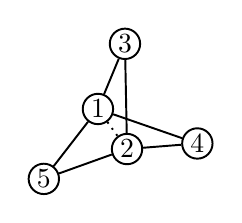
\begin{tikzpicture}
    \node (v1) at (-0.21903373405320625, 0.22955784831048787) {$1$};
    \node (v2) at (0.15063734133854118, -0.27925073637984904) {$2$};
    \node (v3) at (0.12422593618363328, 1.0570054168068603) {$3$};
    \node (v4) at (1.0436598148363205, -0.20848675083938178) {$4$};
    \node (v5) at (-0.90609903369994, -0.6583194825675703) {$5$};
    \draw[dotted] (v1) -- (v2);
    \draw (v1) -- (v3);
    \draw (v1) -- (v4);
    \draw (v1) -- (v5);
    \draw (v2) -- (v3);
    \draw (v2) -- (v4);
    \draw (v2) -- (v5);
    \end{tikzpicture}
  }<4>
  \only{
    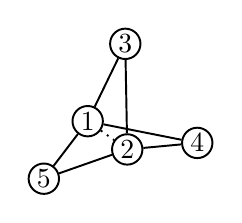
\begin{tikzpicture}
    \node (v1) at (-0.35157196567413607, 0.0701856785098871) {$1$};
    \node (v2) at (0.15071071618961548, -0.2884793992057069) {$2$};
    \node (v3) at (0.12582719661870584, 1.0526711611805561) {$3$};
    \node (v4) at (1.0400325094664926, -0.20562450302182725) {$4$};
    \node (v5) at (-0.9085996316825534, -0.6601362733473835) {$5$};
    \draw[dotted] (v1) -- (v2);
    \draw (v1) -- (v3);
    \draw (v1) -- (v4);
    \draw (v1) -- (v5);
    \draw (v2) -- (v3);
    \draw (v2) -- (v4);
    \draw (v2) -- (v5);
    \end{tikzpicture}
  }<5>
  \only{
    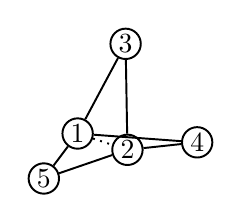
\begin{tikzpicture}
    \node (v1) at (-0.4818361217100955, -0.0909095414938429) {$1$};
    \node (v2) at (0.15078409104068977, -0.2977080620315648) {$2$};
    \node (v3) at (0.12742845705377842, 1.048336905554252) {$3$};
    \node (v4) at (1.0364052040966647, -0.20276225520427274) {$4$};
    \node (v5) at (-0.9111002296651669, -0.6619530641271965) {$5$};
    \draw[dotted] (v1) -- (v2);
    \draw (v1) -- (v3);
    \draw (v1) -- (v4);
    \draw (v1) -- (v5);
    \draw (v2) -- (v3);
    \draw (v2) -- (v4);
    \draw (v2) -- (v5);
    \end{tikzpicture}
  }<6>
  \only{
    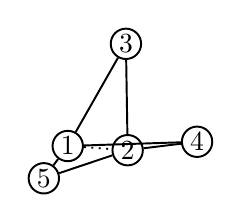
\begin{tikzpicture}
    \node (v1) at (-0.6098262021610849, -0.25372781170070235) {$1$};
    \node (v2) at (0.15085746589176408, -0.3069367248574227) {$2$};
    \node (v3) at (0.129029717488851, 1.0440026499279478) {$3$};
    \node (v4) at (1.0327778987268368, -0.1999000073867182) {$4$};
    \node (v5) at (-0.9136008276477803, -0.6637698549070097) {$5$};
    \draw[dotted] (v1) -- (v2);
    \draw (v1) -- (v3);
    \draw (v1) -- (v4);
    \draw (v1) -- (v5);
    \draw (v2) -- (v3);
    \draw (v2) -- (v4);
    \draw (v2) -- (v5);
    \end{tikzpicture}
  }<7>
  \only{
    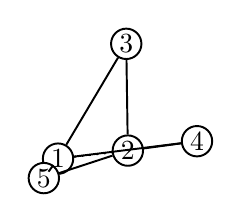
\begin{tikzpicture}
    \node (v1) at (-0.7355422070271043, -0.4182691321106913) {$1$};
    \node (v2) at (0.15093084074283838, -0.3161653876832806) {$2$};
    \node (v3) at (0.13063097792392356, 1.0396683943016436) {$3$};
    \node (v4) at (1.0291505933570089, -0.1970377595691637) {$4$};
    \node (v5) at (-0.9161014256303939, -0.6655866456868227) {$5$};
    \draw[dotted] (v1) -- (v2);
    \draw (v1) -- (v3);
    \draw (v1) -- (v4);
    \draw (v1) -- (v5);
    \draw (v2) -- (v3);
    \draw (v2) -- (v4);
    \draw (v2) -- (v5);
    \end{tikzpicture}
  }<8>
  \only{
    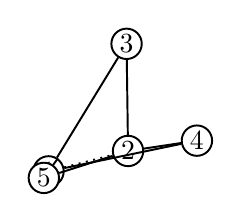
\begin{tikzpicture}
    \node (v1) at (-0.8589841363081532, -0.5845335027238097) {$1$};
    \node (v2) at (0.1510042155939127, -0.3253940505091385) {$2$};
    \node (v3) at (0.1322322383589961, 1.0353341386753394) {$3$};
    \node (v4) at (1.025523287987181, -0.19417551175160913) {$4$};
    \node (v5) at (-0.9186020236130072, -0.6674034364666358) {$5$};
    \draw[dotted] (v1) -- (v2);
    \draw (v1) -- (v3);
    \draw (v1) -- (v4);
    \draw (v1) -- (v5);
    \draw (v2) -- (v3);
    \draw (v2) -- (v4);
    \draw (v2) -- (v5);
    \end{tikzpicture}
  }<9>
  \only{
    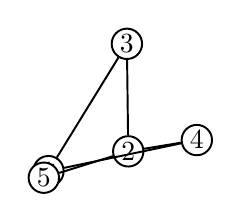
\begin{tikzpicture}
    \node (v1) at (-0.8620532531870092, -0.5859195309528404) {$1$};
    \node (v2) at (0.15107759044498698, -0.3346227133349964) {$2$};
    \node (v3) at (0.1338334987940687, 1.030999883049035) {$3$};
    \node (v4) at (1.021895982617353, -0.19131326393405462) {$4$};
    \node (v5) at (-0.9211026215956206, -0.6692202272464489) {$5$};
    \draw (v1) -- (v3);
    \draw (v1) -- (v4);
    \draw[dotted] (v1) -- (v5);
    \draw (v2) -- (v3);
    \draw (v2) -- (v4);
    \draw (v2) -- (v5);
    \end{tikzpicture}
  }<10>
  \only{
    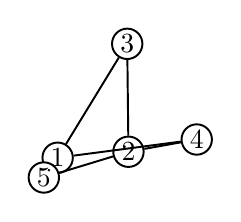
\begin{tikzpicture}
    \node (v1) at (-0.7481606710411273, -0.41984264149308953) {$1$};
    \node (v2) at (0.1511509652960613, -0.34385137616085426) {$2$};
    \node (v3) at (0.13543475922914128, 1.0266656274227308) {$3$};
    \node (v4) at (1.0182686772475251, -0.18845101611650011) {$4$};
    \node (v5) at (-0.9236032195782341, -0.6710370180262621) {$5$};
    \draw (v1) -- (v3);
    \draw (v1) -- (v4);
    \draw[dotted] (v1) -- (v5);
    \draw (v2) -- (v3);
    \draw (v2) -- (v4);
    \draw (v2) -- (v5);
    \end{tikzpicture}
  }<11>
  \only{
    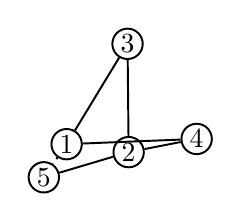
\begin{tikzpicture}
    \node (v1) at (-0.6365421644802156, -0.25204270183020894) {$1$};
    \node (v2) at (0.1512243401471356, -0.3530800389867122) {$2$};
    \node (v3) at (0.13703601966421386, 1.0223313717964266) {$3$};
    \node (v4) at (1.014641371877697, -0.18558876829894558) {$4$};
    \node (v5) at (-0.9261038175608476, -0.6728538088060751) {$5$};
    \draw (v1) -- (v3);
    \draw (v1) -- (v4);
    \draw[dotted] (v1) -- (v5);
    \draw (v2) -- (v3);
    \draw (v2) -- (v4);
    \draw (v2) -- (v5);
    \end{tikzpicture}
  }<12>
  \only{
    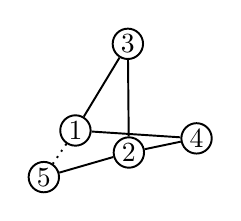
\begin{tikzpicture}
    \node (v1) at (-0.527197733504274, -0.08251971196419894) {$1$};
    \node (v2) at (0.1512977149982099, -0.3623087018125701) {$2$};
    \node (v3) at (0.13863728009928641, 1.0179971161701225) {$3$};
    \node (v4) at (1.011014066507869, -0.18272652048139104) {$4$};
    \node (v5) at (-0.9286044155434611, -0.6746705995858883) {$5$};
    \draw (v1) -- (v3);
    \draw (v1) -- (v4);
    \draw[dotted] (v1) -- (v5);
    \draw (v2) -- (v3);
    \draw (v2) -- (v4);
    \draw (v2) -- (v5);
    \end{tikzpicture}
  }<13>
  \only{
    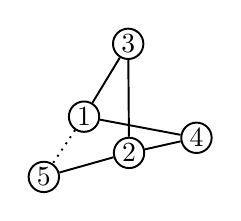
\begin{tikzpicture}
    \node (v1) at (-0.4201273781133026, 0.08872632810494008) {$1$};
    \node (v2) at (0.1513710898492842, -0.37153736463842796) {$2$};
    \node (v3) at (0.14023854053435897, 1.0136628605438183) {$3$};
    \node (v4) at (1.0073867611380412, -0.17986427266383653) {$4$};
    \node (v5) at (-0.9311050135260746, -0.6764873903657014) {$5$};
    \draw (v1) -- (v3);
    \draw (v1) -- (v4);
    \draw[dotted] (v1) -- (v5);
    \draw (v2) -- (v3);
    \draw (v2) -- (v4);
    \draw (v2) -- (v5);
    \end{tikzpicture}
  }<14>
  \only{
    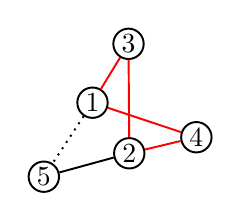
\begin{tikzpicture}
    \node (v1) at (-0.3153310983073013, 0.261695418377209) {$1$};
    \node (v2) at (0.15144446470035852, -0.38076602746428584) {$2$};
    \node (v3) at (0.14183980096943155, 1.009328604917514) {$3$};
    \node (v4) at (1.0037594557682132, -0.177002024846282) {$4$};
    \node (v5) at (-0.9336056115086879, -0.6783041811455145) {$5$};
    \draw[color=red] (v1) -- (v3);
    \draw[color=red] (v1) -- (v4);
    \draw[dotted] (v1) -- (v5);
    \draw[color=red] (v2) -- (v3);
    \draw[color=red] (v2) -- (v4);
    \draw (v2) -- (v5);
    \end{tikzpicture}
  }<15>
\end{frame}

\subsection{Clasificación de $\protect\DynA$ y $\protect\DynD$ por teoría de
gráficas}

\begin{frame}{Motivación}
  Existen algoritmos eficientes que revelan la estructura de gráficas.
  Sólo hay que caracterizar las estructuras que son relevantes para nosotros.
\end{frame}

\begin{frame}{Vértices de corte}
  \begin{definition}<+->[F. Harary -- 1969]
    Sea $G$ una gráfica.
    \begin{itemize}[<+->]
      \item $\kappa\left(G\right)$ denota a la cantidad de componentes conexas 
      de $G$.
      \item $v \in \VertexSet{G}$ es un \alert{vértice de corte} si 
      $\kappa\left(G\right) < \kappa\left(G - v\right)$.
    \end{itemize}
  \end{definition}
  \begin{example}<+->
    \centering
    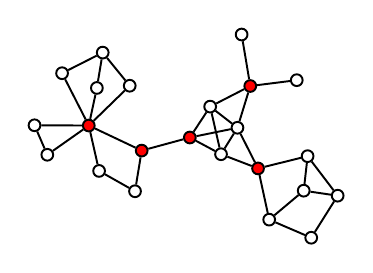
\begin{tikzpicture}
      [every node/.style={circle, draw, inner sep=1.5pt, fill=white}, 
      rotate=-45, scale=0.5]
      \node[fill=red, text=white] (v0) at (-0.81, -3.01) {};
      \node (v1) at (-1.79, -3.98) {};
      \node (v2) at (1.03, -0.49) {};
      \node (v3) at (2.08, -1.15) {};
      \node[fill=red, text=white] (v4) at (1.38, 0.6) {};
      \node (v5) at (0.3, 1.37) {};
      \node[fill=red, text=white] (v6) at (3.0, -0.74) {};
      \node (v7) at (1.9, -0.38) {};
      \node (v8) at (4.12, -1.46) {};
      \node (v9) at (3.67, 0.37) {};
      \node (v10) at (5.2, -1.03) {};
      \node (v11) at (4.92, 0.2) {};
      \node (v12) at (-1.03, -4.28) {};
      \node (v13) at (-1.34, -2.19) {};
      \node (v14) at (4.22, -0.32) {};
      \node (v15) at (2.11, 1.54) {};
      \node (v16) at (0.19, -3.64) {};
      \node (v17) at (-2.23, -2.55) {};
      \node (v18) at (1.2, -3.36) {};
      \node[fill=red, text=white] (v19) at (0.59, -2.51) {};
      \node (v20) at (-0.79, -1.56) {};
      \node (v21) at (-1.87, -1.45) {};
      \node[fill=red, text=white] (v22) at (1.22, -1.41) {};
      \draw (v0) -- (v13);
      \draw (v0) -- (v17);
      \draw (v0) -- (v1);
      \draw (v0) -- (v12);
      \draw (v0) -- (v20);
      \draw (v0) -- (v16);
      \draw (v0) -- (v19);
      \draw (v1) -- (v12);
      \draw (v2) -- (v3);
      \draw (v2) -- (v22);
      \draw (v2) -- (v4);
      \draw (v2) -- (v7);
      \draw (v3) -- (v22);
      \draw (v3) -- (v6);
      \draw (v3) -- (v7);
      \draw (v4) -- (v7);
      \draw (v4) -- (v15);
      \draw (v4) -- (v5);
      \draw (v6) -- (v9);
      \draw (v6) -- (v8);
      \draw (v6) -- (v7);
      \draw (v7) -- (v22);
      \draw (v8) -- (v14);
      \draw (v8) -- (v10);
      \draw (v9) -- (v11);
      \draw (v9) -- (v14);
      \draw (v10) -- (v11);
      \draw (v11) -- (v14);
      \draw (v13) -- (v21);
      \draw (v16) -- (v18);
      \draw (v17) -- (v21);
      \draw (v18) -- (v19);
      \draw (v19) -- (v22);
      \draw (v20) -- (v21);
    \end{tikzpicture}
  \end{example}
\end{frame}

\begin{frame}{Bloques}
  \begin{definitions}[F. Harary -- 1969]
    \begin{itemize}[<+->]
      \item Una gráfica es \alert{inseparable} si no tiene vértices de corte.
      \item Un \alert{bloque} es una subgráfica inseparable que además es 
      maximal respecto a esta propiedad.
      \item El \alert{árbol de bloques} $\BT{G}$ es la gráfica bipartita que 
      contiene una arista $\Set{B, v}$ si y sólo si $B$ es un bloque de $G$ que 
      contiene al vértice de corte $v$.
    \end{itemize}
  \end{definitions}
\end{frame}

\begin{frame}{Árbol de bloques}
  \centering
  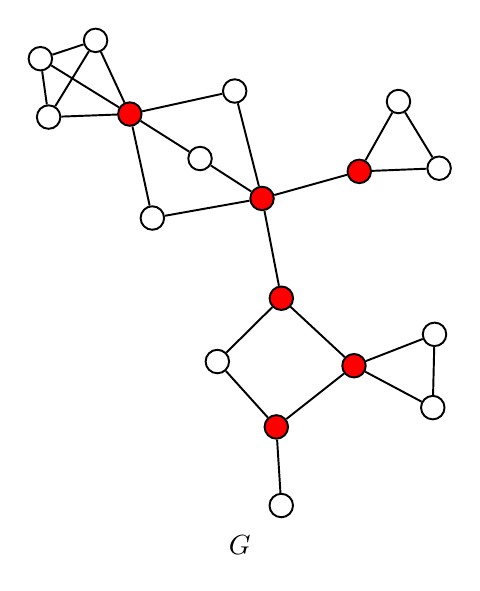
\begin{tikzpicture}[scale=1, every node/.style={inner sep=3pt, circle, 
  draw}]
  \node[fill = red, text = white] (v1) at (4.049900237844199, 
  4.243656972823144) {};
  \node (v2) at (5.063922061379172, 4.2836616692354585) {};
  \node (v3) at (4.547811459396015, 5.130736491076573) {};
  \node[fill = red, text = white] (v4) at (2.8150894862004536, 
  3.8996738525033052) {};
  \node (v5) at (2.468001664314863, 5.264126983902618) {};
  \node[fill = red, text = white] (v6) at (1.1354584570095452, 
  4.971465402433625) {};
  \node (v7) at (0.7010961743248256, 5.90731409966473) {};
  \node (v8) at (0.0, 5.674853511512911) {};
  \node (v9) at (0.10468818559114827, 4.933406411540291) {};
  \node (v10) at (2.027695240309214, 4.4068457745115595) {};
  \node (v11) at (1.4219003207959566, 3.651210810634602) {};
  \node[fill = red, text = white] (v12) at (3.0600275707057074, 
  2.6327164618531254) {};
  \node (v13) at (2.247453971643018, 1.828581489938872) {};
  \node[fill = red, text = white] (v14) at (2.9962205886217443, 
  0.9983347826498138) {};
  \node (v15) at (3.059054256628424, 0.0) {};
  \node[fill = red, text = white] (v16) at (3.9827806990942465, 
  1.7756365046194826) {};
  \node (v17) at (4.983356654966319, 1.2434095884146095) {};
  \node (v18) at (5.00560661216003, 2.1737462632174687) {};
  \draw (v1) -- (v2);
  \draw (v1) -- (v3);
  \draw (v1) -- (v4);
  \draw (v2) -- (v3);
  \draw (v4) -- (v5);
  \draw (v4) -- (v10);
  \draw (v4) -- (v11);
  \draw (v4) -- (v12);
  \draw (v5) -- (v6);
  \draw (v6) -- (v7);
  \draw (v6) -- (v8);
  \draw (v6) -- (v9);
  \draw (v6) -- (v10);
  \draw (v6) -- (v11);
  \draw (v7) -- (v8);
  \draw (v7) -- (v9);
  \draw (v8) -- (v9);
  \draw (v12) -- (v13);
  \draw (v12) -- (v16);
  \draw (v13) -- (v14);
  \draw (v14) -- (v15);
  \draw (v14) -- (v16);
  \draw (v16) -- (v17);
  \draw (v16) -- (v18);
  \draw (v17) -- (v18);
  \node[shape = rectangle, draw = none] (etiqueta) at (2.531961030689586, 
  -0.5) 
  {$G$};
  \end{tikzpicture}
  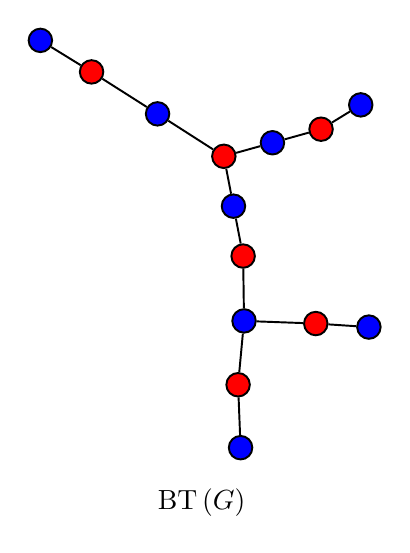
\begin{tikzpicture}[scale = 1, every node/.style={inner sep=3pt, circle, 
    draw, fill=blue}]
  \node (B1) at (4.5538779195397945, 4.552685044378392) {};
  \node (B2) at (0.4853107042313798, 5.371759856287889) {};
  \node (B3) at (1.9736290337260063, 4.438664564797142) {};
  \node (B4) at (3.027637422625084, 0.1991673913249069) {};
  \node (B5) at (4.657247988740198, 1.730930785417187) {};
  \node (B6) at (3.071620707516179, 1.8088173097653235) {};
  \node (B7) at (2.9375585284530805, 3.266195157178215) {};
  \node (B8) at (3.432494862022326, 4.071665412663225) {};
  \node[fill = red, text = white] (v1) at (4.049900237844199, 
  4.243656972823144) {};
  \node[fill = red, text = white] (v4) at (2.8150894862004536, 
  3.8996738525033052) {};
  \node[fill = red, text = white] (v6) at (1.1354584570095452, 
  4.971465402433625) {};
  \node[fill = red, text = white] (v12) at (3.0600275707057074, 
  2.6327164618531254) {};
  \node[fill = red, text = white] (v14) at (2.9962205886217443, 
  0.9983347826498138) {};
  \node[fill = red, text = white] (v16) at (3.9827806990942465, 
  1.7756365046194826) {};
  \draw (B1) -- (v1) -- (B8) -- (v4) -- (B3) -- (v6) -- (B2);
  \draw (v4) -- (B7) -- (v12) -- (B6) -- (v14) -- (B4);
  \draw (B6) -- (v16) -- (B5);
  \node[shape = rectangle, draw = none, fill=none] (etiqueta) at 
  (2.531961030689586, -0.5)
  {$\BT{G}$};
  \end{tikzpicture}
\end{frame}

\begin{frame}{Cómputo de $\BT{G}$}
  \begin{theorem}<+->[J. Hopcroft \& R. Tarjan -- 1971]
    Es posible descomponer una gráfica $G = \Tuple{V, E}$ en sus vértices de 
    corte y bloques en $\bigOh{\abs{V} + \abs{E}}$ operaciones.
  \end{theorem}
  \begin{itemize}[<+->]
    \item Basado en el algoritmo de \alert{recorrido en profundidad}.
  \end{itemize}
\end{frame}

\begin{frame}{Caracterización eficiente para $\DynA$}
  \begin{definition}
    \begin{itemize}[<+->]
      \item Se define la bigráfica $\Full{X}{Y} = \Tuple{X \cup Y, E^+ \cup 
      E^-}$ donde
      \begin{itemize}[<+->]
        \item $E^+ = \binom{X}{2} \cup \binom{Y}{2}$;
        \item $E^- = \BuildSet{\Set{x, y}}{x \in X, y \in Y}$.
      \end{itemize}
      \item $\Fclass$ denota a la clase de todas las bigráficas de la forma 
      $\Full{\cdot}{\cdot}$.
    \end{itemize}
  \end{definition}
  \begin{theorem}<+->
    Una gráfica $G$ es de tipo $\DynA$ si y sólo si cada bloque $B \in \Fclass$ 
    y cada vértice de corte tiene grado 2 en $\BT{G}$.
  \end{theorem}
  \begin{itemize}[<+->]
    \item Demostración autocontenida usando invariantes de flación.
  \end{itemize}
\end{frame}

\begin{frame}{Ejemplo}
  \centering
  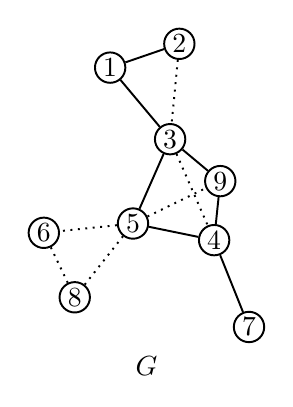
\begin{tikzpicture}[baseline = (caption.base)]
  \node (v1) at (0.045723322887135334, 1.6531597581429232) {$1$};
  \node (v2) at (0.924316069611771, 1.9552990371412833) {$2$};
  \node (v3) at (0.807141212124488, 0.7440631434777515) {$3$};
  \node (v4) at (1.366122335327793, -0.5380224344255913) {$4$};
  \node (v5) at (0.335701115736255, -0.32692551580387064) {$5$};
  \node (v6) at (-0.7967889893835305, -0.4447190885953058) {$6$};
  \node (v7) at (1.809072637133212, -1.6407619146874255) {$7$};
  \node (v8) at (-0.4041868846702505, -1.263837477786485) {$8$};
  \node (v9) at (1.4439611250960338, 0.21170887735943703) {$9$};
  \draw (v1) -- (v2);
  \draw (v1) -- (v3);
  \draw[dotted] (v2) -- (v3);
  \draw[dotted] (v3) -- (v4);
  \draw (v3) -- (v5);
  \draw (v3) -- (v9);
  \draw (v4) -- (v5);
  \draw (v4) -- (v7);
  \draw (v4) -- (v9);
  \draw[dotted] (v5) -- (v6);
  \draw[dotted] (v5) -- (v8);
  \draw[dotted] (v5) -- (v9);
  \draw[dotted] (v6) -- (v8);
  \node[draw = none, shape = rectangle](caption) at (0.5061418238748407, 
  -2.1407619146874257) {$G$};
  \end{tikzpicture}
  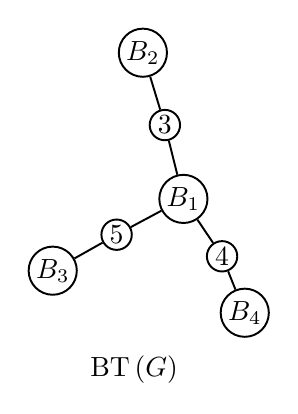
\begin{tikzpicture}[scale = 1.3, baseline = (caption.base)]
  \node (v3) at (0.807141212124488, 0.7440631434777515) {$3$};
  \node (v4) at (1.366122335327793, -0.5380224344255913) {$4$};
  \node (v5) at (0.335701115736255, -0.32692551580387064) {$5$};
  \node (B1) at (0.9882314470711424, 0.022706017651931643) {$B_1$};
  \node (B2) at (0.5923935348744648, 1.4508406462539858) {$B_2$};
  \node (B3) at (-0.2884249194391753, -0.6784940273952205) {$B_3$};
  \node (B4) at (1.5875974862305025, -1.0893921745565085) {$B_4$};
  \draw (B2) -- (v3) -- (B1) -- (v5) -- (B3);
  \draw (B1) -- (v4) -- (B4);
  \node[draw = none, shape = rectangle](caption) at (0.5061418238748407, 
  -1.6407619146874257) {$\BT{G}$};
  \end{tikzpicture}
  \newline
  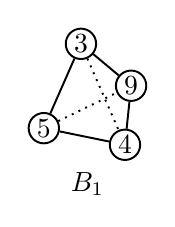
\begin{tikzpicture}[baseline = (caption.base)]
  \node (v3) at (0.807141212124488, 0.7440631434777515) {$3$};
  \node (v4) at (1.366122335327793, -0.5380224344255913) {$4$};
  \node (v5) at (0.335701115736255, -0.32692551580387064) {$5$};
  \node (v9) at (1.4439611250960338, 0.21170887735943703) {$9$};
  \draw[dotted] (v3) -- (v4);
  \draw (v3) -- (v5);
  \draw (v3) -- (v9);
  \draw (v4) -- (v5);
  \draw (v4) -- (v9);
  \draw[dotted] (v5) -- (v9);
  \node[draw = none, shape = rectangle](caption) at (0.8898311204161444, 
  -1.0380224344255913) {$B_1$};
  \end{tikzpicture}
  \begin{tikzpicture}[baseline = (caption.base)]
  \node (v1) at (0.045723322887135334, 1.6531597581429232) {$1$};
  \node (v2) at (0.924316069611771, 1.9552990371412833) {$2$};
  \node (v3) at (0.807141212124488, 0.7440631434777515) {$3$};
  \draw (v1) -- (v2);
  \draw (v1) -- (v3);
  \draw[dotted] (v2) -- (v3);
  \node[draw = none, shape = rectangle](caption) at (0.4850196962494532, 
  0.2440631434777515) {$B_2$};
  \end{tikzpicture}
  \begin{tikzpicture}[baseline = (caption.base)]
  \node (v5) at (0.335701115736255, -0.32692551580387064) {$5$};
  \node (v6) at (-0.7967889893835305, -0.4447190885953058) {$6$};
  \node (v8) at (-0.4041868846702505, -1.263837477786485) {$8$};
  \draw[dotted] (v5) -- (v6);
  \draw[dotted] (v5) -- (v8);
  \draw[dotted] (v6) -- (v8);
  \node[draw = none, shape = rectangle](caption) at (-0.23054393682363775, 
  -1.763837477786485) {$B_3$};
  \end{tikzpicture}
  \begin{tikzpicture}[baseline = (caption.base)]
  \node (v4) at (1.366122335327793, -0.5380224344255913) {$4$};
  \node (v7) at (1.809072637133212, -1.6407619146874255) {$7$};
  \draw (v4) -- (v7);
  \node[draw = none, shape = rectangle](caption) at (1.5875974862305025, 
  -2.1407619146874257) {$B_4$};
  \end{tikzpicture}
\end{frame}

\againframe{ejemploFlacion}

\begin{frame}{Suma de bigráficas}
  \begin{definition}<+->
    $G + H$ es la bigráfica que se obtiene de simplificar la bigráfica 
    $\Tuple{\VertexSet{G} \cup \VertexSet{H}, \EdgeSet{G} + \EdgeSet{H}}$.
  \end{definition}
  \begin{example}<+->
    \centering
    \begin{tikzpicture}[baseline=(current bounding box.center)]
    \node (v1) at (0,0) {$1$};
    \node (v2) at (0, 1) {$2$};
    \node (v3) at (1, 1) {$3$};
    \node (v4) at (2, 1) {$4$};
    \draw (v1) -- (v2) -- (v3) -- (v4);
    \draw[dotted] (v1) -- (v3);
    \node[draw = none, shape = rectangle, fill=none] at (1, -0.5) {$G$};
    \end{tikzpicture}
    \qquad
    \begin{tikzpicture}[baseline=(current bounding box.center)]
    \node (v1) at (0,0) {$1$};
    \node (v3) at (1, 1) {$3$};
    \node (v4) at (2, 1) {$4$};
    \node (v5) at (1, 0) {$5$};
    \draw[dotted] (v1) -- (v5);
    \draw (v1) -- (v3) -- (v5);
    \draw (v3) -- (v4);
    \node[draw = none, shape = rectangle, fill=none] at (1, -0.5) {$H$};
    \end{tikzpicture}
    \qquad
    \begin{tikzpicture}[baseline=(current bounding box.center)]
    \node (v1) at (0,0) {$1$};
    \node (v2) at (0, 1) {$2$};
    \node (v3) at (1, 1) {$3$};
    \node (v4) at (2, 1) {$4$};
    \node (v5) at (1, 0) {$5$};
    \begin{pgfonlayer}{bg}
    \draw (v1) -- (v2) -- (v3) -- (v5);
    \draw[double, double distance=0.5ex] (v3) -- (v4);
    \draw[dotted] (v1) -- (v5);
    \end{pgfonlayer}
    \node[draw = none, shape = rectangle, fill=none] at (1, -0.5) {$G + H$};
    \end{tikzpicture}
  \end{example}
\end{frame}

\begin{frame}{Invariante para $\BT{G}$}
  \begin{lemma}<+->
    Sea $\Set{s, r}$ una arista de alguna $H \in \Fclass$, y sea $F\in 
    \Fclass$  tal que $\VertexSet{F} \cap \VertexSet{H} = \Set{s}$;
    entonces $T_{s\, r}\left(F + H\right) = F^{\prime} + H^{\prime}$ donde:
    \begin{enumerate}[<+->]
      \item $F^{\prime}$ y $H^{\prime}$ son miembros de $\Fclass$ tales que 
      $\VertexSet{F^{\prime}} \cap \VertexSet{H^{\prime}} = \Set{s}$
      \item $F^{\prime} -r = F$ y $H - r = H^{\prime}$.
    \end{enumerate}
  \end{lemma}
\end{frame}

\begin{frame}{Ejemplo}
  \centering
  \begin{tikzpicture}[baseline=(caption.base), scale=0.67]
  \node (s) at (1, 1) {$s$};
  \node (r) at (3, 1) {$r$};
  \node (x) at (2, 2) {$x$};
  \node (y) at (2, 0) {$y$};
  \node (xp) at (0, 2) {$z$};
  \node (yp) at (0, 0) {$w$};
  \draw (xp) -- (yp) -- (s) -- (r) -- (x) -- (y) -- (s);
  \draw[dotted] (xp) -- (s) -- (x);
  \draw[dotted] (y) -- (r);
  \node[draw=none, fill=none, rectangle](caption) at (1.5, -1) {
    $\underbrace{\Full{\Set{s, z}}{\Set{w}}}_{F} + 
    \underbrace{\Full{\Set{s, x}}{\Set{r, y}}}_{H}$
  };
  \end{tikzpicture}
  \qquad
  \begin{tikzpicture}[baseline=(caption.base), scale=0.67]
  \node (s) at (2, 1) {$s$};
  \node (r) at (0, 1) {$r$};
  \node (x) at (3, 2) {$x$};
  \node (y) at (3, 0) {$y$};
  \node (xp) at (1, 2) {$z$};
  \node (yp) at (1, 0) {$w$};
  \draw (r) -- (yp) -- (s) -- (y) -- (x);
  \draw (yp) -- (xp);
  \draw[dotted] (s) -- (r) -- (xp) -- (s) -- (x);
  \node[draw=none, fill=none, rectangle](caption) at (1.5, -1) {
    $\underbrace{\Full{\Set{r, s, z}}{\Set{w}}}_{F^\prime} + 
    \underbrace{\Full{\Set{s, x}}{\Set{y}}}_{H^\prime}$
  };
  \end{tikzpicture}
\end{frame}

\begin{frame}{Construcción para $\DynD$}
  \begin{block}{Construcción (pegado de $\DynD$-núcleo)}
    \textbf{Datos:}
    \begin{itemize}[<+->]
      \item Una bigráfica cíclica con vértices $x_1, \ldots, x_h$ ($h \ge 2$) 
      que satisface la condición de ciclo (el \alert{$\DynD$-núcleo}).
      \item Bigráficas $F_1, F_2, \ldots, F_h$, tales que:
      \begin{itemize}
        \item cada $F_i$ tiene tipo Dynkin $\DynA$ y contiene una arista 
        $\Set{x_i, x_{i + 1}}$ con el mismo estilo de línea que en $H$;
        \item $x_{i}$ y $x_{i + 1}$ son vértices internos de $F_i$
        \item todas las $F_i$ son disjuntas por vértices excepto por aquellos 
        que conforman el $\DynD$-núcleo.
      \end{itemize}
    \end{itemize}
    \textbf{Procedimiento:}
    \begin{enumerate}[<+->]
      \item Calcular la suma de bigráficas $\sum_{i = 1}^{h} F_i$; a la 
      bigráfica resultante le llamamos el \alert{pegado de $\DynD$-núcleo de 
      $H$ y $F_{1},  F_{2}, \ldots, F_{h}$}.
    \end{enumerate}
  \end{block}
\end{frame}

\begin{frame}{Ejemplo de pegado de $\DynD$-núcleo}
  \centering
  \begin{tikzpicture}[scale=0.75]
  \node (v1) at (3.0150114830736507, 3.129003623971734) {$1$};
  \node (v2) at (3.917079755406643, 2.2958693914572956) {$2$};
  \node (v8) at (3.9884807418820447, 3.309312509002968) {$8$};
  \draw[dotted] (v1) -- (v2);
  \draw[dotted] (v1) -- (v8);
  \draw[dotted] (v2) -- (v8);
  \node[shape = rectangle, draw = none](caption) at (3.5017461124778477, 
  1.7958693914572956) {$F_1$};
  \end{tikzpicture}
  \qquad
  \begin{tikzpicture}[scale=0.75]
  \node (v2) at (3.917079755406643, 2.2958693914572956) {$2$};
  \node (v3) at (3.4024115411863685, 1.2283971864666778) {$3$};
  \node (v6) at (4.451017709784681, 1.3362103274209054) {$6$};
  \node (v7) at (5.344841430338816, 0.6541539788363036) {$7$};
  \draw (v2) -- (v3);
  \draw[dotted] (v2) -- (v6);
  \draw (v3) -- (v6);
  \draw (v6) -- (v7);
  \node[shape = rectangle, draw = none](caption) at (4.373626485762593, 
  0.15415397883630355) {$F_2$};
  \end{tikzpicture}
  \qquad
  \begin{tikzpicture}[scale=0.75]
  \node (v3) at (3.4024115411863685, 1.2283971864666778) {$3$};
  \node (v4) at (2.154169208821005, 1.4754766802019228) {$4$};
  \draw[dotted] (v3) -- (v4);
  \node[shape = rectangle, draw = none](caption) at (2.778290375003687, 
  0.7283971864666778) {$F_3$};
  \end{tikzpicture}
  \qquad
  \begin{tikzpicture}[scale=0.75]
  \node (v4) at (2.154169208821005, 1.4754766802019228) {$4$};
  \node (v5) at (1.9575540985303148, 2.3923457340900125) {$5$};
  \node (v9) at (1.2487588329811672, 1.1784184772829662) {$9$};
  \node (v10) at (1.0845840387201626, 2.2164645086290857) {$10$};
  \node (v11) at (0.0, 2.7225958691745493) {$11$};
  \node (v12) at (0.2552709377085125, 0.48507729902362406) {$12$};
  \node (v13) at (1.0178209040429833, 0.0) {$13$};
  \draw[dotted] (v4) -- (v5);
  \draw[dotted] (v4) -- (v9);
  \draw (v4) -- (v10);
  \draw[dotted] (v5) -- (v9);
  \draw (v5) -- (v10);
  \draw (v9) -- (v10);
  \draw (v9) -- (v12);
  \draw (v9) -- (v13);
  \draw (v10) -- (v11);
  \draw[dotted] (v12) -- (v13);
  \node[shape = rectangle, draw = none](caption) at (1.0770846044105025, 
  -0.5) {$F_4$};
  \end{tikzpicture}
  \qquad
  \begin{tikzpicture}[scale=0.75]
  \node (v1) at (3.0150114830736507, 3.129003623971734) {$1$};
  \node (v5) at (1.9575540985303148, 2.3923457340900125) {$5$};
  \draw (v1) -- (v5);
  \node[shape = rectangle, draw = none](caption) at (2.4862827908019827, 
  1.8923457340900125) {$F_5$};
  \end{tikzpicture}
  \qquad
  \begin{tikzpicture}[scale=0.75]
  \node[fill = green, text = white] (v1) at (3.0150114830736507, 
  3.129003623971734) {$\boldsymbol{1}$};
  \node[fill = green, text = white] (v2) at (3.917079755406643, 
  2.2958693914572956) {$\boldsymbol{2}$};
  \node[fill = green, text = white] (v3) at (3.4024115411863685, 
  1.2283971864666778) {$\boldsymbol{3}$};
  \node[fill = green, text = white] (v4) at (2.154169208821005, 
  1.4754766802019228) {$\boldsymbol{4}$};
  \node[fill = green, text = white] (v5) at (1.9575540985303148, 
  2.3923457340900125) {$\boldsymbol{5}$};
  \draw[dotted] (v1) -- (v2);
  \draw (v1) -- (v5);
  \draw (v2) -- (v3);
  \draw[dotted] (v3) -- (v4);
  \draw[dotted] (v4) -- (v5);
  \node[shape = rectangle, draw = none](caption) at (2.937316926968479, 
  0.7283971864666778) {$H$};
  \end{tikzpicture}
  \qquad
  \begin{tikzpicture}[scale=0.75]
  \node[fill = green, text = white] (v1) at (3.0150114830736507, 
  3.129003623971734) {$\boldsymbol{1}$};
  \node[fill = green, text = white] (v2) at (3.917079755406643, 
  2.2958693914572956) {$\boldsymbol{2}$};
  \node[fill = green, text = white] (v3) at (3.4024115411863685, 
  1.2283971864666778) {$\boldsymbol{3}$};
  \node[fill = green, text = white] (v4) at (2.154169208821005, 
  1.4754766802019228) {$\boldsymbol{4}$};
  \node[fill = green, text = white] (v5) at (1.9575540985303148, 
  2.3923457340900125) {$\boldsymbol{5}$};
  \node (v6) at (4.451017709784681, 1.3362103274209054) {$6$};
  \node (v7) at (5.344841430338816, 0.6541539788363036) {$7$};
  \node (v8) at (3.9884807418820447, 3.309312509002968) {$8$};
  \node (v9) at (1.2487588329811672, 1.1784184772829662) {$9$};
  \node (v10) at (1.0845840387201626, 2.2164645086290857) {$10$};
  \node (v11) at (0.0, 2.7225958691745493) {$11$};
  \node (v12) at (0.2552709377085125, 0.48507729902362406) {$12$};
  \node (v13) at (1.0178209040429833, 0.0) {$13$};
  \draw[dotted] (v1) -- (v2);
  \draw (v1) -- (v5);
  \draw[dotted] (v1) -- (v8);
  \draw (v2) -- (v3);
  \draw[dotted] (v2) -- (v6);
  \draw[dotted] (v2) -- (v8);
  \draw[dotted] (v3) -- (v4);
  \draw (v3) -- (v6);
  \draw[dotted] (v4) -- (v5);
  \draw[dotted] (v4) -- (v9);
  \draw (v4) -- (v10);
  \draw[dotted] (v5) -- (v9);
  \draw (v5) -- (v10);
  \draw (v6) -- (v7);
  \draw (v9) -- (v10);
  \draw (v9) -- (v12);
  \draw (v9) -- (v13);
  \draw (v10) -- (v11);
  \draw[dotted] (v12) -- (v13);
  \node[shape = rectangle, draw = none](caption) at (2.672420715169408, 
  -0.5) {$G$};
  \end{tikzpicture}
\end{frame}

\begin{frame}{Observaciones acerca del pegado de $\DynD$-núcleo}
  El pegado de $\DynD$-núcleo\ldots\pause
  \begin{itemize}[<+->]
    \item caracteriza al tipo $\DynD$;
    \item define la estructura de la bigráfica, no de la gráfica subyacente;
    \item considera al $\DynA$-espejo es un caso especial, cuando $h = 2$;
    \item tiene demostración autocontenida basada en invariante de flación.
  \end{itemize}
\end{frame}

\begin{frame}{Casos del invariante de flación para $\DynD$}
  \begin{tikzpicture}[baseline = (current bounding box.center)]
  \node[fill = green, text = white] (v1) at (-0.17702807361217932, 
  0.2169077993202585) {$\boldsymbol{1}$};
  \node[fill = green, text = white] (v2) at (0.5094847697505441, 
  -0.6140803384090112) {$\boldsymbol{2}$};
  \node (v3) at (0.6069997477997765, 0.7096309089544152) {$3$};
  \node (v4) at (1.1343769499172704, 0.10036276119312261) {$4$};
  \node (v5) at (-0.648145832261598, -0.8701436995030774) {$5$};
  \node (v6) at (-1.4270078527724706, -1.5265337186469214) {$6$};
  \draw (v1) -- (v3);
  \draw (v1) -- (v4);
  \draw (v1) -- (v5);
  \draw[dotted] (v2) -- (v3);
  \draw[dotted] (v2) -- (v4);
  \draw (v2) -- (v5);
  \draw[dotted] (v3) -- (v4);
  \draw (v5) -- (v6);
  \end{tikzpicture}
  \pause{}$\overset{T_{5 \, 6}}{\longmapsto}$
  \begin{tikzpicture}[baseline = (current bounding box.center)]
  \node[fill = green, text = white] (v1) at (1.0252371598281498, 
  1.5047159922868778) {$\boldsymbol{1}$};
  \node[fill = green, text = white] (v2) at (1.5722710209957673, 
  0.8123465644435764) {$\boldsymbol{2}$};
  \node (v3) at (1.7791313280577472, 2.0813745224256897) {$3$};
  \node (v4) at (2.2965614513501706, 1.458351047878916) {$4$};
  \node (v5) at (0.2956250391481165, 0.8626071897560861) {$5$};
  \node (v6) at (0.8077603377334521, 0.24445137916669574) {$6$};
  \draw (v1) -- (v3);
  \draw (v1) -- (v4);
  \draw (v1) -- (v5);
  \draw (v1) -- (v6);
  \draw[dotted] (v2) -- (v3);
  \draw[dotted] (v2) -- (v4);
  \draw (v2) -- (v5);
  \draw (v2) -- (v6);
  \draw[dotted] (v3) -- (v4);
  \draw[dotted] (v5) -- (v6);
  \end{tikzpicture}
  \pause{}$\overset{T_{1 \, 5}}{\longmapsto}$
  \begin{tikzpicture}[baseline = (current bounding box.center)]
  \node[fill = green, text = white] (v1) at (0.20349457991430148, 
  1.055913409132112) {$\boldsymbol{1}$};
  \node[fill = green, text = white] (v2) at (1.3755446374420803, 
  0.34426344565076855) {$\boldsymbol{2}$};
  \node (v3) at (0.9235745895584886, 1.707922024213706) {$3$};
  \node (v4) at (1.626496864221418, 1.3141116166259303) {$4$};
  \node (v5) at (0.9715951986840659, 0.9729584162837188) {$5$};
  \node (v6) at (0.2615442503405679, -0.15873666360225455) {$6$};
  \draw (v1) -- (v3);
  \draw (v1) -- (v4);
  \draw[dotted] (v1) -- (v5);
  \draw (v1) -- (v6);
  \draw[dotted] (v2) -- (v3);
  \draw[dotted] (v2) -- (v4);
  \draw (v2) -- (v5);
  \draw (v2) -- (v6);
  \draw[dotted] (v3) -- (v4);
  \draw (v3) -- (v5);
  \draw (v4) -- (v5);
  \end{tikzpicture}
  
  \pause{}$\overset{T_{3 \, 1}}{\longmapsto}$
  \begin{tikzpicture}[baseline = (current bounding box.center)]
  \node[fill = green, text = white] (v1) at (-0.2814306111671281, 
  0.8990219271931051) {$\boldsymbol{1}$};
  \node[fill = green, text = white] (v2) at (0.75691323601581, 
  0.8600382799848384) {$\boldsymbol{2}$};
  \node[fill = green, text = white] (v3) at (0.5586925858271716, 
  1.7274992556341786) {$\boldsymbol{3}$};
  \node (v4) at (1.6988576401743483, 1.1678621669884481) {$4$};
  \node (v5) at (1.4035768281579486, 1.9530041708564487) {$5$};
  \node (v6) at (0.12280539183944258, -0.09186288489949457) {$6$};
  \draw[dotted] (v1) -- (v2);
  \draw[dotted] (v1) -- (v3);
  \draw (v1) -- (v6);
  \draw[dotted] (v2) -- (v3);
  \draw[dotted] (v2) -- (v4);
  \draw (v2) -- (v5);
  \draw (v2) -- (v6);
  \draw[dotted] (v3) -- (v4);
  \draw (v3) -- (v5);
  \draw (v4) -- (v5);
  \end{tikzpicture}
  \pause{}$\overset{T_{2 \, 3}}{\longmapsto}$
  \begin{tikzpicture}[baseline = (current bounding box.center)]
  \node[fill = green, text = white] (v1) at (0.14005101347942864, 
  0.12855941484799926) {$\boldsymbol{1}$};
  \node (v2) at (1.2212373161957064, 1.0733183866926967) {$2$};
  \node[fill = green, text = white] (v3) at (0.3015747050465922, 
  1.8535846558746634) {$\boldsymbol{3}$};
  \node (v4) at (2.391858784671201, 0.91610215943802) {$4$};
  \node (v5) at (2.1662309211727266, 1.8121513857833453) {$5$};
  \node (v6) at (0.4164932553705382, 0.8121665822901439) {$6$};
  \draw[dotted] (v1) -- (v2);
  \draw (v1) -- (v6);
  \draw (v2) -- (v3);
  \draw[dotted] (v2) -- (v4);
  \draw (v2) -- (v5);
  \draw (v2) -- (v6);
  \draw[dotted] (v3) -- (v6);
  \draw (v4) -- (v5);
  \end{tikzpicture}
\end{frame}

\subsection{Un algoritmo polinomial para la clasificación 
$\protect\DynA$-$\protect\DynD$-$\protect\DynE$}

\begin{frame}{Motivación}
  En computación se considera que un problema es tratable cuando existe un 
  algoritmo que lo resuelve en tiempo polinomial.
\end{frame}

\begin{frame}{Observaciones}
  \begin{itemize}[<+->]
    \item Sea $G$ una bigráfica conexa y definida positiva de $n$ vértices.
    \item $G$ no puede tener aristas múltiples por ser definida positiva.
    \item Si $n > 8$ entonces $G$ es de tipo $\DynA$ o $\DynD$.
    \item Si $n \le 8$ entonces el algoritmo de las inflaciones puede 
    determinar su tipo en $\bigOh{1}$ operaciones.
  \end{itemize}
\end{frame}

\begin{frame}{Algoritmo propuesto}
  \begin{block}{Algoritmo}
    \SetKwFunction{FnDynkin}{Dynkin}
    \begin{algorithm}[H]
      \Function{\FnDynkin{$\mat{A}$}}{
        \KwIn{Una matriz casi-Cartan simétrica $\mat{A}$}
        verificar que $\mat{A}$ es definida positiva y salir si no lo es\;
        \ForEach{componente conexa $K$ de $\Bigraph{\mat{A}}$}{
          \uIf{$K$ tiene $n \le 8$ vértices}{
            usar el algoritmo de las inflaciones en $K$ para calcular su 
            tipo Dynkin e imprimirlo\;
          }
          \Else{
            Analizar si $K$ tiene tipo Dynkin $\DynA$ o $\DynD$ e imprimir el 
            resultado\;
          }
        }
      }
    \end{algorithm}
  \end{block}
\end{frame}

\begin{frame}{Paso 1}
  \framesubtitle{Determinar si una matriz $\mat{A} \in \sqCclass$ es definida 
  positiva usando sólo números enteros}
  No se puede hacer en tiempo polinomial usando el método de Gauss:
  \begin{equation*}
  \begin{bmatrix}2 & -1\\
  -1 & 2 & -1\\
  & -1 & \ddots & \ddots\\
  &  & \ddots & 2 & -1\\
  &  &  & -1 & 2
  \end{bmatrix}\mapsto\begin{bmatrix}2 & -1\\
  & 4 & -2\\
  &  & \ddots & \ddots\\
  &  &  & 2^{2^{n-2}} & -2^{\left(2^{n-2}-1\right)}\\
  &  &  &  & 2^{2^{n-1}}
  \end{bmatrix}
  \end{equation*}
\end{frame}

\begin{frame}{Paso 1}
  \begin{block}<+->{Algoritmo (adaptación de E. Bareiss -- 1968)}
    \SetKwFunction{DefinidaPositiva}{definida\_positiva}
    \begin{algorithm}[H]
      \Function{\DefinidaPositiva{$\mat{A}$}}{
        \For{$k=1$ \KwTo $n$}{
          \lIf{$\entry{\mat{A}}{k}{k} \le 0$}{\Return \textsc{Falso}}
          \For{$i=k + 1$ \KwTo $n$}{
            \For{$j=k + 1$ \KwTo $n$}{
              $\entry{\mat{A}}{i}{j} \gets \det
              \begin{bmatrix}
              \entry{\mat{A}}{k}{k} & \entry{\mat{A}}{k}{j}\\
              \entry{\mat{A}}{i}{k} & \entry{\mat{A}}{i}{j}
              \end{bmatrix}$\;
              \lIf{$k > 1$}{$\entry{\mat{A}}{i}{j} \gets 
                \frac{\entry{\mat{A}}{i}{j}}{\entry{\mat{A}}{k - 1}{k - 1}}$}
            }
          }
        }
      }
      \Return \textsc{Verdadero}
    \end{algorithm}
  \end{block}
\end{frame}

\begin{frame}{Características del algoritmo de Bareiss}
  \begin{itemize}[<+->]
    \item Justificado por el criterio de Sylvester dado que al final de la 
    iteración $i$, $\entry{\mat{A}}{i}{i} = \det\left(\mat{A}^{\Tuple{i, 
    i}}\right)$.
    \item Complejidad $\bigOh{n^5\left(L + \log n\right)^2}$ donde $2^L \ge 
    \max_{i, j}\abs{\entry{\mat{A}}{i}{j}}$.
   \item En nuestro caso $L = 2$: entonces existe un algoritmo polinomial.
  \end{itemize}
\end{frame}

\appendix

\section*{Apéndice}

\subsection*{Lecturas complementarias}
\begin{frame}[allowframebreaks]{Lecturas complementarias}

\beamertemplatebookbibitems
\begin{thebibliography}{1}
%\bibitem{Autor1990}A. Autor. \newblock\emph{Manual de Lo que sea}.\newblock
%Editorial, 1990.\beamertemplatearticlebibitems

\bibitem{Abarca2016}M. Abarca \& D. Rivera\newblock Graph Theoretical and 
Algorithmic Characterizations of Positive Definite Symmetric Quasi-Cartan 
Matrices\emph{.}
\newblock\emph{Fundamenta Informaticae}. 149(3):241--261, 2016.

\bibitem{Barot1999}M. Barot.\newblock A characterization of positive unit 
forms\emph{.}
\newblock\emph{Boletín de la Sociedad Matemática Mexicana}. 5:87--94, 1999.

\bibitem{Barot2001}M. Barot.\newblock A characterization of positive unit 
forms, part II\emph{.}
\newblock\emph{Boletín de la Sociedad Matemática Mexicana}. 7:13--22, 2001.

\end{thebibliography}
\end{frame}
\end{document}
